%%%%%%%%%%%%%%%%%%%%%%%%%%%%%%%%%%%%%%%%%%%%%%%%%%%%%%%%%%%%%%%%%%%%%%%%%%%%%%%
%%
%%          $Id: Rulebook.tex 2014-12-12 balkce $
%%    author(s): RoboCupAtHome Technical Committee(s)
%%  description: introduction to RoboCupAtHome
%%
%%%%%%%%%%%%%%%%%%%%%%%%%%%%%%%%%%%%%%%%%%%%%%%%%%%%%%%%%%%%%%%%%%%%%%%%%%%%%%%
\documentclass[11pt, twoside, openright, a4paper, chapterprefix]{scrbook}
\usepackage[inner=2.5cm, outer=2.5cm, top=4cm, bottom=4cm]{geometry}

%%% PACKAGES %%%%%%%%%%%%%%%%%%%%%%%%%%%%%%%%%%%%%%%%%%%%%%%%%%%%%%%%%%%%%%%%%%
%%%%%%%%%%%%%%%%%%%%%%%%%%%%%%%%%%%%%%%%%%%%%%%%%%%%%%%%%%%%%%%%%%%%%%%%%%%%%%%
%%
%%          $Id: packages.tex 385 2013-02-12 21:53:10Z holz $
%%    author(s): RoboCupAtHome Technical Committee(s)
%%  description: List of packages for the RoboCupAtHome rulebook
%%
%%%%%%%%%%%%%%%%%%%%%%%%%%%%%%%%%%%%%%%%%%%%%%%%%%%%%%%%%%%%%%%%%%%%%%%%%%%%%%%
\usepackage{soul}

\usepackage[english]{babel}
\usepackage{amsmath,amssymb,amsfonts}
\usepackage[nice]{nicefrac}
\usepackage{siunitx}
\usepackage{graphicx}
\usepackage{multicol}
\usepackage{verbatim}
\usepackage{fancyhdr}
% \usepackage{svn-multi}
\usepackage{color}
\usepackage{xcolor,colortbl}
\usepackage{epsfig}
\usepackage{makeidx}
\usepackage{lscape}
\usepackage{picinpar}
% \usepackage{./styles/bar}
\usepackage{./styles/tweaklist}
%\usepackage{subfigure}
\usepackage{enumerate,paralist}
\usepackage{multirow}
\usepackage{pgffor}
\usepackage{array}
\usepackage{etoolbox}
\usepackage{hyperref}
\usepackage{tabularx}
\usepackage{xspace}
\usepackage{csquotes}
\usepackage[inline]{enumitem}

%\usepackage[utf8x]{inputenc}
%\usepackage{times}
%\usepackage{helvet}
%\usepackage{courier}

\usepackage{url}
\usepackage{caption}
%\usepackage{subcaption}
\usepackage{epstopdf}
\usepackage{subfig}
\usepackage{float}
\usepackage{wrapfig}
%\usepackage{titlesec}
\usepackage{xfrac}

% Local Variables:
% TeX-master: "../Rulebook"
% End:

\usepackage[titletoc]{appendix}
\usepackage{enumitem}
\usepackage{mathtools}
\usepackage{gensymb}
\setlist{noitemsep}

%%% SubfigureSetup %%%%%%%%%%%%%%%%%%%%%%%%%%%%%%%%%%%%%%%%%%%%%%%%%%%%%%%%%%%%
%\renewcommand{\subfigtopskip}{5pt}        % default is 10pt
%\renewcommand{\subfigbottomskip}{5pt}     % default is 10pt
%\renewcommand{\subfigcapskip}{3pt}        % default is 10pt
%\renewcommand{\subfigcapmargin}{7pt}      % default is 10pt

%%% TweakList-Setup %%%%%%%%%%%%%%%%%%%%%%%%%%%%%%%%%%%%%%%%%%%%%%%%%%%%%%%%%%%
\renewcommand{\itemhook}{%                 % modify itemize-spacing
  \setlength{\topsep}{2pt}%
  \setlength{\partopsep}{1pt}%
  \setlength{\itemsep}{-1pt}%
}
\renewcommand{\enumhook}{%                 % modify enumerate-spacing
  \setlength{\topsep}{2pt}%
  \setlength{\partopsep}{1pt}%
  \setlength{\itemsep}{-1pt}%
}
\renewcommand{\descripthook}{%             % modify description-spacing
  \setlength{\topsep}{2pt}%
  \setlength{\partopsep}{1pt}%
  \setlength{\itemsep}{-1pt}%
}

\setkomafont{title}{\normalfont}
\setkomafont{sectioning}{\normalfont\bfseries}
\addtokomafont{caption}{\small}
\setkomafont{captionlabel}{\small\bfseries}
\setkomafont{descriptionlabel}{\normalfont\bfseries}
\renewcommand*{\chapterformat}{\LARGE{Chapter \thechapter}}

%%% MACROS %%%%%%%%%%%%%%%%%%%%%%%%%%%%%%%%%%%%%%%%%%%%%%%%%%%%%%%%%%%%%%%%%%%%
\newcommand{\YEAR}{2019}
\newcommand{\STATE}{Draft}
% \newcommand{\STATE}{Final}
%
% Local Variables:
% TeX-master: "../Rulebook"
% End:

\graphicspath{{\YEAR/}{./images/}}
%%%%%%%%%%%%%%%%%%%%%%%%%%%%%%%%%%%%%%%%%%%%%%%%%%%%%%%%%%%%%%%%%%%%%%%%%%%%%%%
%%
%%          $Id: macros.tex 399 2013-02-14 20:24:02Z holz $
%%    author(s): RoboCupAtHome Technical Committee(s)
%%  description: Macros for the RoboCupAtHome rulebook
%%
%%%%%%%%%%%%%%%%%%%%%%%%%%%%%%%%%%%%%%%%%%%%%%%%%%%%%%%%%%%%%%%%%%%%%%%%%%%%%%%

%%%%%%%%%%%%%%%%%%%%%%%%%%%%%%%%%%%%%%%%%%%%%%%%%%%%%%%%%%%%%%%%%%%%
% Macros for generating score sheets for RoboCup@Home              %
% to be used in the rulebook or during the competition             %
%                                                                  %
% Author: Dirk Holz & David Gossow                                 %
% Modif : Mauricio Matamoros                                       %
% $Id: macros_score_sheets.tex 429 2013-04-30 10:09:55Z holz $     %
%%%%%%%%%%%%%%%%%%%%%%%%%%%%%%%%%%%%%%%%%%%%%%%%%%%%%%%%%%%%%%%%%%%%


\usepackage{calc}
\usepackage{ifthen}
\usepackage{wasysym}
\usepackage{chngpage}


%%% Counters / temp. variables %%%%%%%%%%%%%%%%%

\newcounter{currTestScore}
\newcounter{currTestScoreTotal}
\newcounter{currTestScoreTotalWithoutBonus}
\newcounter{currOutstandingBonus}
\newcommand{\scorelistOptions}{}
\newcommand{\scoresheetOptions}{}

% set \shortScoresheet to true for the rulebook version and to false for the referee's scoresheet
\newcommand{\shortScoresheet}{true}

% set \threeAttempts to true for three columns in the scoresheet
\newcommand{\threeAttempts}{false}

% set \retryAvailable to true for a second column in the scoresheet
\newcommand{\retryAvailable}{true}

% set \continueAvailable to true for CONTINUE sections
\newcommand{\continueAvailable}{true}

% set \dataRecordingBonus to true for data recording bonus
\newcommand{\dataRecordingBonus}{false}

% name of the current test, is set automatically in the rulebook
\newcommand{\currentTest}{}

% (internal) if-clause shortcut to switch between short rulebook version and full score sheet for referees
\newcommand{\ifShortScoresheet}[2]{%
  \ifthenelse{ \equal{\shortScoresheet}{true}}{%
    #1%
  }{%
    #2%
  }%
}

\newcommand{\ifEvaluationSheet}[2]{%
  \ifthenelse{ \equal{\scoresheetOptions}{evaluationSheet}}{%
    #1%
  }{%
    #2%
  }%
}

% (internal) draws the scoresheet line for score handwritting
\newcommand{\scoreline}[1][0.08]{\rule{#1\linewidth}{.2pt}}

% (internal) draws the lines for score hadndwritting in the table outline based on the number of attempts
\newcommand{\attemptScoreLines}{
  \switchAttempts
    {\scoreline[0.06] & \scoreline[0.06] & \scoreline[0.06]}
    {\scoreline & \scoreline}
    {\scoreline}
}

% (internal) Select one of the provided arguments based on the number of attempts
% (3 tries, retry (2) or only try (1))
\newcommand{\switchAttempts}[3]{
  \ifthenelse{\equal{\threeAttempts}{true}}{#1}{\ifthenelse{\equal{\retryAvailable}{true}}{#2}{#3}}
}

% (internal) stores the number of attempts to perform
\edef\numAttempts{0}
% (internal) writes on the command \numAttempts the number of attempts to perform
\newcommand\defNumAttempts{
  \switchAttempts
  {\global\edef\numAttempts{3}}
  {\global\edef\numAttempts{2}}
  {\global\edef\numAttempts{1}}
}

%% commands for overriding internal calculations %%%%%%%%%%%%%%%%%%%%%%%%%%%%%%%%%%%%%%%%

% set score counter to arbitrary value
\newcommand{\setTotalScore}[1]%
{%
  \setcounter{currTestScore}{#1}
}

% set outstanding bonus to arbitrary value
\newcommand{\setOutstandingBonus}[1]%
{%
  \setcounter{currOutstandingBonus}{#1}
}




%% Score sheet page layout %%%%%%%%%%%%%%%%%%%%%%%%%%%%%%%%%%%%%%%%%%%%%%%%%%%%%%%%%%%%%%%%

% usage: \begin{scoresheet}[repeatable] ... \end{scoresheet}
\newenvironment{scoresheet}[1][]{
  % begin
  \newpage

  \renewcommand{\scoresheetOptions}{#1}

  \begin{minipage}[t]{0.8\textwidth}%
    \vspace{0pt}
    {\huge \textbf{Score Sheet} }

    \vspace{2 em}

    \begin{tabular}{ @{} l l l}
      \textbf{Test:} & \currentTest \\[.9 em]

      \ifEvaluationSheet{}{%
        \textbf{Team name:} & \scoreline[0.6]\\[.9 em]%
      }%
      %
      \textbf{Referee name:} & \scoreline[0.6]\\[.9 em]%
      %
      %	\ifEvaluationSheet{}{%
      %   \textbf{Restart:} & \Square ~1st try \hspace{1 em} \Square ~2nd try
      %	}
      %
      % test repetition checkboxes (for stage 2 tests)
      \ifthenelse{ \equal{#1}{repeatable} }{%
	\textbf{Test repetition:} & \Square ~1st \hspace{1 em} \Square ~2nd\\[.9em]%
      }{}
    \end{tabular}

    \vspace{0.5 em}

  \end{minipage}
  \hfill
  \begin{minipage}[t]{0.15\textwidth}%
    \vspace{0pt}
    
\includegraphics[width=\textwidth]{images/logo_RoboCupAtHome.jpg}%
  \end{minipage}\\
}
{
  % end
  \vspace{.2 em}
  \textbf{Remarks:}

  %% signatures of referee / team leader %%%%%%%%%%%%
  \vfill
  \ifEvaluationSheet{
    % team evaluation sheet
    \begin{tabular}{@{} @{\extracolsep{\fill}} l l @{}}
      \scoreline[0.25] \hspace{0.05\linewidth} & \scoreline[0.25] \hspace{0.05\linewidth}
      \\
      \textit{Date \& time}%
      & \textit{Referee}
    \end{tabular}
  }{
    % normal sheet
    \begin{tabular}{@{} @{\extracolsep{\fill}} l l l @{}}
      \scoreline[0.25] \hspace{0.05\linewidth} & \scoreline[0.25] \hspace{0.05\linewidth} & \scoreline[0.25]
      \\
      \textit{Date \& time}%
      & \textit{Referee} %
      & \textit{Team leader}
    \end{tabular}
  }

  \newpage
}


%% Score list table %%%%%%%%%%%%%%%%%%%%%%%%%%%%%%%%%%%%%%%%%%%%%%%%%%%%%%%%%%%%%%%%

% usage: \begin{scorelist}[openDoorSignal] ... \end{scorelist}
\newenvironment{scorelist}[1][]{
  % begin

  % init variables %%%%%%%%%
  \renewcommand{\scorelistOptions}{#1}
  \setcounter{currTestScore}{0}
  \setcounter{currOutstandingBonus}{0}

  % setup table %%%%%%%%%
  \vspace{0.8 em}

  \ifShortScoresheet {
    \begin{tabular*}{\textwidth}{@{} @{\extracolsep{\fill}} p{0.8\linewidth} r @{}}
      \ifEvaluationSheet{
        \textbf{Team} & \textbf{Score} \\ \hline
      }{%
        \textbf{Action} & \textbf{Score} \\ \hline
      }
    }{
      % else:
      % \begin{tabular*}{\textwidth}{@{}p{0.65\linewidth}lp{0.15\linewidth}@{}}
      %   \textbf{Action} & \textbf{Score} & \multicolumn{1}{l}{\textbf{Success}}\\ \hline
      \ifEvaluationSheet{
        \begin{tabular*}{\textwidth}{@{} @{\extracolsep{\fill}} p{0.7\linewidth} r r @{}}
          \textbf{Team} & \textbf{Score} & \textbf{Result}\\ \hline
        }{
          \ifthenelse{\equal{\threeAttempts}{true}}{
            \begin{tabular*}{\textwidth}{@{} @{\extracolsep{\fill}} p{0.6\linewidth} r r r r @{}}
            \textbf{Action} & \textbf{Score} & \textbf{\small $1^{st}$ try} & \textbf{\small $2^{nd}$ try} & \textbf{\small$3^{rd}$ try} \\ \hline
          }
          %else
          {
            \begin{tabular*}{\textwidth}{@{} @{\extracolsep{\fill}} p{0.6\linewidth} r r r @{}}
            \textbf{Action} & \textbf{Score} \ifthenelse{\equal{\retryAvailable}{true}}{& \textbf{1st try} & \textbf{2nd try}}{ & \textbf{Only try}} \\ \hline
          }
        }
      }
    }
      {
        % end

	\ifEvaluationSheet{}{%

          % calculate max. score, outstanding bonus %%%%%%%
          \ifthenelse{\value{currOutstandingBonus} = 0}{%
            \setcounter{currOutstandingBonus}{ \value{currTestScore} / 10 }
          }{}
          \setcounter{currTestScoreTotal}{ \value{currTestScore} + \value{currOutstandingBonus} }
          \setcounter{currTestScoreTotalWithoutBonus}{ \value{currTestScore} }


          % Special penalties & bonuses %%%%%%%%%%%%%%%%
          \scoreheading{Special penalties \& standard bonuses}

          \ifthenelse {\equal{\dataRecordingBonus}{true}}{\scoreitem{10}{Contributing with recorded data ($\frac{\sum gathered\ points}{max\ points} \times$) \ifShortScoresheet{(see sec.~\ref{rule:datarecording})}{}}}{}

          \scoreitem{-50}{Not attending \ifShortScoresheet{(see sec.~\ref{rule:not_attending})}{}}

          \ifthenelse{\equal{\scorelistOptions}{openDoorSignal}}{
            \scoreitem{-10}{Using start button \ifShortScoresheet{(see sec.~\ref{rule:start_button})}{}}
          }{}

          % \ifthenelse{\value{currOutstandingBonus} = 0}{
          \scoreitem{\thecurrOutstandingBonus}{Outstanding performance \ifShortScoresheet{(see sec.~\ref{rule:outstanding_performance})}{}}
          % }{}

          % Total score %%%%%%%%%%%%%%%%
          \hline\\
          % \textbf{Total score} & \scoring{ \thecurrTestScoreTotal } %
          \ifShortScoresheet {%
            % No Score per try in short version
          }{%
            \textbf{\textit{Score per try}} & \scoring{ \thecurrTestScoreTotalWithoutBonus } %
          }
          % add line to put in total:
          \ifShortScoresheet{}{& \attemptScoreLines} \\
          \ifShortScoresheet{
            \textbf{Total score} (excluding penalties and bonuses) & \scoring{ \thecurrTestScoreTotalWithoutBonus } %
          }{
            \defNumAttempts
            & \\
            \textbf{Total score}  & \scoring{ \thecurrTestScoreTotalWithoutBonus } & \multicolumn{\numAttempts}{c}{\scoreline[0.20]}
          } \\
	}

      \end{tabular*}

    }


    %% Score sheet table entries %%%%%%%%%%%%%%%%%%%%%%%%%%%%%%%%%%%%%%%%%%%%%%%%%%%%%%%%%%%%%%%%

    % for loop helper
    % usage: \forloop[step]{counter}{initial_value}{conditional}{code_block}
    \newcommand{\forloop}[5][1]%
    {%
      \setcounter{#2}{#3}%
      \ifthenelse{#4}%
      {%
 	#5%
 	\addtocounter{#2}{#1}%
 	\forloop[#1]{#2}{\value{#2}}{#4}{#5}%
      }%
      % else
      {%
      }%
    }

    \newcounter{ct}

    % heading
    % usage: \scoreheading{text}
    \newcommand{\scoreheading}[1]{
      \ifShortScoresheet {%
        \phantom{.} \\[-4 ex] \multicolumn{2}{@{}l}{\textbf{\textit{#1}}}\\[0pt]
      }{%
        \phantom{.} \\[-4 ex] \multicolumn{3}{@{}l}{\textbf{\textit{#1}}}\\[0pt]
      }
    }

    % table entry
    % usage: \scoreitem[multiplicity]{points}{description}
    \newcommand{\scoreitem}[3][1]{

      % add to max. total score if points > 0
      \ifthenelse{ #2 > 0 }{
        \addtocounter{currTestScore}{ #2 * #1 }
      }{}%
      %
      \begin{minipage}[t]{\linewidth} {#3} \vspace{0.1 em} \end{minipage} & %
      \scoring{ \ifthenelse{ \equal{#1}{1} }{}{ #1 $\times$} \ifthenelse{ \equal{#2}{0} }{}{ #2}}%
      % insert check marks:
      %	\ifShortScoresheet{}{ & \forloop{ct}{0}{\value{ct} < #1}{ \Square}} \\[3pt]
      % insert line
      \ifShortScoresheet{ %
        \\
      }{ % else
        \ifEvaluationSheet{}{& \attemptScoreLines} \\[0pt]
      }
    }


% Local Variables:
% TeX-master: "../Rulebook"
% End:

%%%%%%%%%%%%%%%%%%%%%%%%%%%%%%%%%%%%%%%%%%%%%%%%%%%%%%%%%%%%%%%%%%%%%%%%%%%%%%%
%%
%%          $Id: macros_open_demonstrations.tex 391 2013-02-14 07:57:07Z sugiura $
%%    author(s): holz
%%  description: simple macros for specifications of open challenges
%%
%%%%%%%%%%%%%%%%%%%%%%%%%%%%%%%%%%%%%%%%%%%%%%%%%%%%%%%%%%%%%%%%%%%%%%%%%%%%%%%

\newcommand{\OpenDemonstrationTask}[2] {
  \begin{enumerate}%
    \item \textbf{Setup and demonstration:} The team has a maximum of \timing{#1 minutes} for setup, presentation and demonstration.%
    \item \textbf{Interview and cleanup:} After the demonstration, there is
	      another \timing{#2 minutes} where the team answers %
    questions by the jury members.\\%
    During the interview time, the team has to undo its changes to the environment.%
  \end{enumerate}%
}

\newcommand{\OpenDemonstrationChanges}{
  \subsection{Changes to the environment}
  \begin{enumerate}
    \item \textbf{Making changes:} As in the other open demonstrations, teams are allowed to make modifications to the arena as they like, 
    but under the condition that they are reversible.
    \item \textbf{Undoing changes:} In the interview and cleanup team, changes need to be made undone by the team. 
    The team has to leave the arena in the \emph{very same} condition they entered it.
  \end{enumerate}
}
% Local Variables:
% TeX-master: "../Rulebook"
% End:

%%%%%%%%%%%%%%%%%%%%%%%%%%%%%%%%%%%%%%%%%%%%%%%%%%%%%%%%%%%%%%%%%%%%%%%%%%%%%%%
%%
%%          $Id: macros_leagues.tex 399 2017-06-04 13:36:00Z matamoros $
%%    author(s): RoboCupAtHome Technical Committee(s)
%%  description: Macros for the RoboCupAtHome rulebook
%%
%%%%%%%%%%%%%%%%%%%%%%%%%%%%%%%%%%%%%%%%%%%%%%%%%%%%%%%%%%%%%%%%%%%%%%%%%%%%%%%
\ifdefined\league
\else%
    % Provided for compatibility with older versions
    \newcommand\teamsListFile{teams/teams.tex}
    \newcommand{\league}{}
    \newcommand{\leagueFullName}{}
\fi

%% Import team from the Open Standard Platform League %%%%%%%%%%% %%
\ifthenelse{\equal{\league}{OPL}}{
    \newcommand\teamsListFile{teams/OPL.tex}
    \newcommand{\leagueFullName}{Open Platform League}
}{}

%% Import team from the Domestic Standard Platform League %%%%%%% %%
\ifthenelse{\equal{\league}{DSPL}}{
    \newcommand\teamsListFile{teams/DSPL.tex}
    \newcommand{\leagueFullName}{Domestic Standard Platform League}
}{}

%% Import team from the Social Standard Platform League %%%%%%%%% %%
\ifthenelse{\equal{\league}{SSPL}}{
    \newcommand\teamsListFile{teams/SSPL.tex}
    \newcommand{\leagueFullName}{Social Standard Platform League}
}{}


%% %%%%%%%%%%%%%%%%%%%%%%%%%%%%%%%%%%%%%%%%%%%%%%%%%%%%%%%%%%%%%% %%
%%  Per league macros                                             %%
%% %%%%%%%%%%%%%%%%%%%%%%%%%%%%%%%%%%%%%%%%%%%%%%%%%%%%%%%%%%%%%% %%

%% Domestic Standard Platform League %%%%%%%%%%%%%%%%%%%%%%%%%%%% %%
\newcommand{\ifDSPL}[1]{
    \ifthenelse{\equal{\league}{} \OR \equal{\league}{DSPL}}{#1}{}
}

\newcommand{\ifNotDSPL}[1]{
    \ifthenelse{\equal{\league}{} \OR \equal{\league}{OPL} \OR \equal{\league}{SSPL}}{#1}{}
}


%% Open Platform League %%%%%%%%%%%%%%%%%%%%%%%%%%%%%%%%%%%%%%%%% %%
\newcommand{\ifOPL}[1]{
    \ifthenelse{\equal{\league}{} \OR \equal{\league}{OPL}}{#1}{}
}

\newcommand{\ifNotOPL}[1]{
    \ifthenelse{\equal{\league}{} \OR \equal{\league}{DSPL} \OR \equal{\league}{SSPL}}{#1}{}
}


%% Open Standard Platform League %%%%%%%%%%%%%%%%%%%%%%%%%%%%%%%% %%
\newcommand{\ifSSPL}[1]{
    \ifthenelse{\equal{\league}{} \OR \equal{\league}{SSPL}}{#1}{}
}

\newcommand{\ifNotSSPL}[1]{
    \ifthenelse{\equal{\league}{} \OR \equal{\league}{OPL} \OR \equal{\league}{DSPL}}{#1}{}
}

% \newcommand{\ifLeague}[2]{
%     \ifNotSSPL{#1}
%     \ifSSPL{#2}
% }




%% %%%%%%%%%%%%%%%%%%%%%%%%%%%%%%%%%%%%%%%%%%%%%%%%%%%%%%%%%%%%%% %%
%%  List of teams import macro                                    %%
%% %%%%%%%%%%%%%%%%%%%%%%%%%%%%%%%%%%%%%%%%%%%%%%%%%%%%%%%%%%%%%% %%

\newcommand{\loadTeamsListFile}{%
    \input{\teamsListFile}
}

% \expandafter\expandafter\newcommand\TEAMSSTAGEONE{\csname TEAMS\league \endcsname}

% Local Variables:
% TeX-master: "../Rulebook"
% End:

\newcommand{\rulebookVersion}{\STATE\ version for RoboCup \YEAR\xspace(\VERSION)}

\def\RoboCup{{\textsc{RoboCup}}}
\def\Robocup{{\textsc{RoboCup}}}
\def\robocup{{\textsc{RoboCup}}}
\def\AtHome{{\textsc{RoboCup@Home}}}
\def\MSL{\textsc{Middle Size League}}
\def\MS{{\textsc{Middle Size}}}
\def\SSL{\textsc{Soccer Simulation League}}
\def\SS{\textsc{Soccer Simulation}}

\def\TC{technical committee (TC)}
\def\OC{organizing committee (OC)}

\newcommand{\textbi}[1]{\textbf{\textit{#1}}}
\renewcommand{\labelenumi}{\arabic{enumi}.}
\renewcommand{\labelenumii}{\labelenumi\arabic{enumii}.}
\renewcommand{\labelenumiii}{\labelenumii.\arabic{enumiii}.}


%% %%%%%%%%%%%%%%%%%%%%%%%%%%%%%%%%%%%%%%%%%%%%%%%%%%%%%%%%% %%
%%                    Developement-Tools                     %%
%% %%%%%%%%%%%%%%%%%%%%%%%%%%%%%%%%%%%%%%%%%%%%%%%%%%%%%%%%% %%

%% %%%%%%%%%%%%%%%%%%%%%%%%%%%%%%%%%%%%%%%
\newcommand{\tbc}[1]{\textbf{\it\color{red}{t.b.c. ...}#1\color{black}}}
\newcommand{\todo}[1]{\textbf{\it\color{red}{todo: }#1\color{black}}}
\newcommand{\TODO}[1]{\textbf{\it\color{red}{TODO:\\}#1\color{black}}}
\newcommand{\chk}[1]{\textbf{\color{red}#1\color{black}}}

\newcommand{\reworkon}{\marginpar{\raggedright\color{red}{$\downarrow$rework}\color{black}}}
\newcommand{\reworkoff}{\marginpar{\raggedright\color{red}{$\uparrow$rework}\color{black}}}

%% %%%%%%%%%%%%%%%%%%%%%%%%%%%%%%%%%%%%%%%
%%  site notes/margin notes
\def\note#1{\marginpar{\raggedright\tiny#1}}
\def\mpar#1{\marginpar{\raggedright\tiny#1}}
\def\rand#1{\marginpar{\raggedright\tiny#1}}
\setlength{\marginparwidth}{2cm}

\newcommand{\refsec}[1]{Section~\ref{#1}}
\newcommand{\reftab}[1]{Table~\ref{#1}}
\newcommand{\reffig}[1]{Figure~\ref{#1}}

%% %%%%%%%%%%%%%%%%%%%%%%%%%%%%%%%%%%%%%%%
%% side-annotation-macros for easy lookup
% \newcommand{\awardmark}{\marginpar{\centering\includegraphics[width=.34cm]{images/icon_award.pdf}}}
% \newcommand{\refmark}{\marginpar{\centering\includegraphics[width=.5cm]{images/icon_whistle.pdf}}}
% \newcommand{\referee}[1]{\emph{#1}\marginpar{\centering\includegraphics[width=.5cm]{images/icon_whistle.pdf}}}
% \newcommand{\scoremark}{\marginpar{\centering\includegraphics[width=.34cm]{images/icon_score.pdf}}}
\newcommand{\awardmark}{}
\newcommand{\refmark}{}
\newcommand{\referee}[1]{}
\newcommand{\scoremark}{}
%\newcommand{\scoring}[1]{\emph{#1}\marginpar{\centering\includegraphics[width=.34cm]{images/icon_score.pdf}}}
\newcommand{\scoring}[1]{\emph{#1}}
\newcommand{\timark}{\marginpar{\centering\includegraphics[width=.34cm]{icon_clock.pdf}}}

%\newcommand{\timing}[1]{\emph{#1}\marginpar{\centering\includegraphics[width=.34cm]{images/icon_clock.pdf}}}
\newcommand{\timing}[1]{\emph{#1}}

\def\svnRevision{Unknown} %
\def\svnChangeData{Unknown} %
\def\revnumtmpfile{.temp_ruleook_version}
\def\revdattmpfile{.temp_ruleook_date}
\immediate\write18{git rev-list HEAD | wc -l > \revnumtmpfile}
%\immediate\write18{svnversion . > \revnumtmpfile}
\IfFileExists{\revnumtmpfile}{\def\svnRevision{\input{\revnumtmpfile}\unskip}}{}
\immediate\write18{git log -1 --date=short  | grep 'Date:' | awk '{print $2}'> \revdattmpfile}
%\immediate\write18{svn info | grep 'Last Changed Date:' | awk '{print $4}'> \revdattmpfile}
\IfFileExists{\revdattmpfile}{\def\svnChangeData{\input{\revdattmpfile}\unskip}}{}
% \IfFileExists{\revnumtmpfile}{\immediate\write18{rm -f \revnumtmpfile}}{}
% \IfFileExists{\revdattmpfile}{\immediate\write18{rm -f \revdattmpfile}}{}
\newcommand{\VERSION}{Revision \svnChangeData\_\svnRevision}


% Local Variables:
% TeX-master: "../Rulebook"
% End:

%% %%%%%%%%%%%%%%%%%%%%%%%%%%%%%%%%%%%%%%%%%%%%%%%%%%%%%%%%%%%%%%%%%%%%%%%%%%%
%%
%%          $Id: abbrevix.tex 373 2013-02-12 20:32:49Z holz $
%%    author(s): RoboCupAtHome Technical Committee(s)
%%  description: Abbreviations for the RoboCupAtHome RuleBook
%%
%% %%%%%%%%%%%%%%%%%%%%%%%%%%%%%%%%%%%%%%%%%%%%%%%%%%%%%%%%%%%%%%%%%%%%%%%%%%%

%% temp-variables %%%%%%%%%
\newlength{\adxtemp}
\newlength{\adxspace}
\setlength{\adxspace}{3cm}

%% %%%%%%%%%%%%%%%%%%%%%%%%%%%%%%%%%%%%%%%
%%  Commands to use this
%% %%%%%%%%%%%%%%%%%%%%%%%%%%%%%%%%%%%%%%%

%% \abb{abk}
%% to reference an abbreviation
\newcommand{\abb}[1]{\hypertarget{#1}{#1}}

%% \term{the term}
%% print 'the term' in italic,
%% do not include 'the term' in index
%\newcommand{\term}[1]{#1\index{#1}}
\newcommand{\term}[1]{\textit{#1}}

%% \iterm{the term}
%% print 'the term' in italic,
%% include 'the term' in index
\newcommand{\iterm}[1]{\textit{#1}\index{#1}}

%% \nterm{the term}
%% do NOT print 'the term' but include 'the term' in index
\newcommand{\nterm}[1]{\index{#1}}

%% \TERM
%% print first term, add second term to index
\newcommand{\Term}[2]{\textit{#1}\index{#2}}


%% \aterm{the term}{abb}
%% print 'term', 
%% include 'term' with abbreviation 'abb' in abbreviation-index
\newcommand{\aterm}[2]{\settowidth{\adxtemp}{#2}{\hypertarget{#2}{#1 (#2)}\abbex{#2\hspace{\adxspace}\hspace{-\the\adxtemp}#1}}}

%% \iaterm{the term}{abbreviation} 
%% print 'term', 
%% include 'the term' in index, 
%% and include abbreviation in abbreviation-index
\newcommand{\iaterm}[2]{\settowidth{\adxtemp}{#2}{\hypertarget{#1}{\textit{#1} (#2)}\index{#1}\abbex{#2\hspace{\adxspace}\hspace{-\the\adxtemp}#1}}}

%% %%%%%%%%%%%%%%%%%%%%%%%%%%%%%%%%%%%%%%%
%%  Main Abbreviation Definitions
%% %%%%%%%%%%%%%%%%%%%%%%%%%%%%%%%%%%%%%%%

\makeatletter
\newlength{\QZ@TOChdent}% Used to define hanging indents.
\setlength{\QZ@TOChdent}{1.0em}%
\renewcommand{\@pnumwidth}{1.55em}%
\makeatother
%
%\newenvironment{simpleenv}[4]{\clearpage}{\clearpage}%
%\newenvironment{simpleenv}[4]{\clearpage}{\pagebreak}%
\newenvironment{simpleenv}[4]{\pagebreak}{\pagebreak}%
\newcommand{\BaseDiff}{0}%
%\newcommand{\RSpnum}[1]{\makebox[\@pnumwidth][r]{#1}}%
\newcommand{\RSpnum}[1]{\makebox[1.57em][r]{#1}}%
\newcommand{\RSnopnum}[1]{\makebox[\@pnumwidth][r]{}}%
\newcommand{\RSpset}[1]{\RSpnum{#1}}%
%
\newcommand{\printabbex}[4][\jobname]{%
  \typeout{ ***** printabbex #1 #2 #3 #4 for file \jobname.tex}%
  \IfFileExists{#1.and}{%
     \begin{simpleenv}{#1}{#2}{#3}{#4}%
       \pagestyle{plain} %
       \addcontentsline{toc}{chapter}{#2}%
       \chapter*{\textbf{#3}}{#4}%
       \input{#1.and}%
       \vfill%
     \end{simpleenv}%
   }%
   {\typeout{ ***** ERROR: No file #1.and found for file \jobname.tex.}}}%
\renewcommand{\see}[2]{#2 \emph{see} #1}%
\makeatletter
\newcommand{\makeabbex}[1][\jobname]{\begingroup
  \makeatletter
  \if@filesw \expandafter\newwrite\csname #1@adxfile\endcsname
  \expandafter\immediate\openout \csname #1@adxfile\endcsname #1.adx\relax
  \typeout{ ***** Writing abbex file #1.adx for file \jobname.tex.}%
  \fi \endgroup}
%\makeatother
%\makeatletter
\@onlypreamble{\makeindex}%
\newcommand{\abbex}[2][\jobname]{\@bsphack\begingroup
               \def\protect##1{\string##1\space}\@sanitize
               \@wrabbex{#1}{#2}}
\newcommand{\@wrabbex}[2]{\let\thepage\relax
   \xdef\@gtempa{\@ifundefined{#1@adxfile}{}{\expandafter
      \write\csname #1@adxfile\endcsname{\string
      \indexentry{#2|}{\thepage}}}}\endgroup\@gtempa
   \if@nobreak \ifvmode\nobreak\fi\fi\@esphack}
\makeatother
\newcommand{\indxspace}{\par\vspace{\BaseDiff\baselineskip}}
\makeatletter
\newcommand{\IndexSet}{%
\renewcommand{\@idxitem}{\par\setlength{\leftskip}{0pt}%
                         \setlength{\hangindent}{\QZ@TOChdent}}%
\renewcommand{\subitem}{\par\setlength{\leftskip}{0.25in}%
                         \setlength{\hangindent}{\QZ@TOChdent}}%
\renewcommand{\subsubitem}{\par\setlength{\leftskip}{0.5in}%
                         \setlength{\hangindent}{\QZ@TOChdent}}%
\renewcommand{\indexspace}{}
\renewcommand{\indxspace}{\par\vspace{\BaseDiff\baselineskip}}
\renewenvironment{theindex}{%
                \setlength{\parindent}{\z@}%
                \parskip\z@ \@plus .3\p@\relax
                \setlength{\rightskip}{\@tocrmarg}%
                \setlength{\parfillskip}{-\rightskip}%
                \let\item\@idxitem}
} %% End of the IndexSet definition
\makeatother

\newcommand{\printidx}{\addcontentsline{toc}{chapter}{Index}\printindex}
\newcommand{\printabx}{\printabbex{Abbreviations}{Abbreviations}{}}
%\newcommand{\printabbrevidx}{\printindex[abb]{Abk�rzungen}{Abk�rzungen}{}}
\newcommand{\printabbrevidx}{\printabbex{Abbreviations}{Abbreviations}{}}
%\newcommand{\makeabbrevidx}{\makeindex[abb]}
\newcommand{\makeabbrevidx}{\makeabbex}

% Local Variables:
% TeX-master: "../Rulebook"
% End:




\makeindex                                % generate index
\makeabbex                                % generate abbreviations

%%% DOCUMENTINFO %%%%%%%%%%%%%%%%%%%%%%%%%%%%%%%%%%%%%%%%%%%%%%%%%%%%%%%%%%%%%%
\hypersetup{
  pdftitle     = {RoboCup@Home Rules and Regulations},
  pdfsubject   = {RoboCup@Home Rulebook},
  pdfauthor    = {RoboCup@Home Technical Committee},
  pdfkeywords  = {RoboCup, @Home, Rules, Competition},
  colorlinks   = true,
  anchorcolor  = blue,
  linkcolor    = blue,
  urlcolor     = blue,
}

%%% HEADINGS & PAGE STYLE %%%%%%%%%%%%%%%%%%%%%%%%%%%%%%%%%%%%%%%%%%%%%%%%%%%%%
\newcommand{\footline}{RoboCup@Home Rulebook / \rulebookVersion}
\pagestyle{fancy}
\renewcommand{\chaptermark}[1]{\markboth{\chaptername\ \thechapter. \ #1}{}}
\renewcommand{\sectionmark}[1]{\markright{\thesection \ #1}{}\renewcommand{\currentTest}{#1}}
\fancyhf{}
\fancyhead[LE,RO]{\thepage}
\fancyhead[RE]{\sffamily\rightmark}
\fancyhead[LO]{\sffamily\leftmark}
\fancyfoot[C]{\scriptsize \sffamily \footline{}}
\fancypagestyle{plain}{
        \fancyhf{}
        \fancyhead[LE,RO]{\thepage}
        \fancyhead[RE]{\sffamily\rightmark}
        \fancyhead[LO]{\sffamily\leftmark}
        \fancyfoot[C]{\scriptsize \sffamily \footline{}}
		\renewcommand{\headrulewidth}{0.5 pt}
}
\fancypagestyle{empty}{
        \fancyhf{}
        \fancyhead{}
        \fancyfoot[C]{\scriptsize \sffamily \footline{}}
		\renewcommand{\headrulewidth}{0 pt}
}

%\newcommand{\sectionbreak}{\clearpage}
%\newcommand{\subsectionbreak}{\clearpage}


%%%%%%%%%%%%%%%%%%%\renewcommand{%%%%%%%%%%%%%%%%%%%%%%%%%%%%%%%%%%%%%%%%%%%%%%%%%%%%%%%%%%%%
%%%%%%%%%%%%%%%%%%%%%%%%%%%%%%%%%%%%%%%%%%%%%%%%%%%%%%%%%%%%%%%%%%%%%%%%%%%%%%%
%%%%%%%%%%%%%%%%%%%%%%%%%%%%%%%%%%%%%%%%%%%%%%%%%%%%%%%%%%%%%%%%%%%%%%%%%%%%%%%

\begin{document}

%% %%%%%%%%%%%%%%%%%%%%%%%%%%%%%%%%%%%%%%%%%%%%%%%%%%%%%%%%%%%%%%%%%%%%%%%%%%%
%%
%%          $Id: titlepage.tex 428 2013-04-30 10:01:14Z holz $
%%    author(s): RoboCupAtHome Technical Committee(s)
%%  description: Title page for the RoboCupAtHome RuleBook
%%
%% %%%%%%%%%%%%%%%%%%%%%%%%%%%%%%%%%%%%%%%%%%%%%%%%%%%%%%%%%%%%%%%%%%%%%%%%%%%
\begin{titlepage}
  \begin{center}
    {
      
\includegraphics[width=.25\textwidth]{images/logo_RoboCupFed.jpg}
      \hfill
      
\includegraphics[width=.25\textwidth]{images/logo_RoboCupAtHome.jpg}\\[1.23ex]
    }
    \vspace{2.7 cm}
    \hrulefill\par
    {%
      \vspace*{.27cm}
      \Huge{RoboCup@Home}\\[1.23ex]
      \Large Rules \& Regulations \\[2ex]
    }
    \hrulefill\par
    \vfill
    ~~ Version: \YEAR ~~Rev-\svnRevision ~~ \\
    ~~ Last Build Date: \today \quad Time: \the\time ~~ \\
    ~~ Last Revision Date: \svnChangeData ~~ %\\
    %\vfill
  \end{center}
\end{titlepage}
% Local Variables:
% TeX-master: "../Rulebook"
% End:


\pagestyle{empty}
%% %%%%%%%%%%%%%%%%%%%%%%%%%%%%%%%%%%%%%%%%%%%%%%%%%%%%%%%%%%%%%%%%%%%%%%%%%%%
%%
%%          $Id: acknowledgments.tex 404 2013-02-15 08:51:20Z sugiura $
%%    author(s): RoboCupAtHome Technical Committee(s)
%%  description: Acknowledgments for the RoboCupAtHome RuleBook
%%
%% %%%%%%%%%%%%%%%%%%%%%%%%%%%%%%%%%%%%%%%%%%%%%%%%%%%%%%%%%%%%%%%%%%%%%%%%%%%



\section*{About this rulebook}
This is the official rulebook of the RoboCup@Home competition \YEAR.
It has been written by the \YEAR ~RoboCup@Home Technical Committee with the special collaboration of (in alphabetical order):
% Mauricio Matamoros,
% and
% Loy van Beek.



\section*{How to cite this rulebook}
If you refer to RoboCup@Home and this rulebook in particular, please cite:

Mauricio Matamoros, Caleb Rascon, Justin Hart, Dirk Holz, Kai Chen, and Loy van Beek.
\enquote{Robocup@Home \YEAR: Rule and regulations,}
\url{http://www.robocupathome.org/rules/2019_rulebook.pdf}, \YEAR.

\begin{center}
\begin{minipage}{0.8\textwidth}
	\footnotesize%
	\verbatiminput{citation.bib}
\end{minipage}
\end{center}

\section*{Acknowledgments}
\label{sec:acknowledgments}
We would like to thank the members of the technical committee who put up the rules and the organizing committee who organizes the competition.

~\\\noindent People that have been working on this rulebook as member of one of the league's committees (in alphabetical order):
\begin{center}
\begin{minipage}{0.8\textwidth}
\begin{multicols}{3}%
\footnotesize
\noindent%

% Kai Chen\\
% Justin Hart\\
% Luca Iocchi\\
% Mauricio Matamoros\\
% Dirk Holz\\
% \columnbreak
% Raphael Memmesheimer\\
% Alexander Moriarty\\
% Caleb Rascon\\
% Sammy Pfeiffer\\
% \columnbreak
% Komei Sugiura\\
% Sven Wachsmuth\\
% Tijn van der Zant\\
\end{multicols}
\end{minipage}
\end{center}

We also like to thank all the people who contributed to the RoboCup@Home league with their feedback and comments.

~\\\noindent People that have been working on this rulebook as member the league (in alphabetical order):
\begin{center}
\begin{minipage}{0.8\textwidth}
\begin{multicols}{2}%
\footnotesize
\noindent%
% Loy van Beek (@LoyVanBeek)\\
% Sebastian Meyer zu Borgsen (@semeyerz)\\
% Matthijs van der Burgh (@MatthijsBurgh)\\
% Remi Fabre (@RemiFabre)\\
% Tarik Kelestemur (@tkelestemur)\\
% \columnbreak%
% Johannes Kummert (@johaq)\\
% Florian Lier (@warp1337)\\
% Hiroyuki Okada (@okadahiroyuki)\\
% @AMR-\\
% @fibonatic\\
\end{multicols}
\end{minipage}
\end{center}


% Local Variables:
% TeX-master: "../Rulebook"
% End:

\clearpage

\pagestyle{empty}
\tableofcontents
\clearpage

\pagestyle{plain}

%% %%%%%%%%%%%%%%%%%%%%%%%%%%%%%%%%%%%%%%%%%%%%%%%%%%%%%%%%%%%%%%%%%%%%%%%%%%%
%%
%%    author(s): RoboCupAtHome Technical Committee(s)
%%  description: Introduction
%%
%% %%%%%%%%%%%%%%%%%%%%%%%%%%%%%%%%%%%%%%%%%%%%%%%%%%%%%%%%%%%%%%%%%%%%%%%%%%%
\chapter{Introduction}
\label{chap:introduction}


\section{RoboCup}
\iterm{RoboCup} is an international joint project to promote AI, robotics, and related fields. It is an attempt to foster AI and intelligent robotics research by providing standard problems where a wide range of technologies can be integrated and examined. More information can be found at http://www.robocup.org/.

\section{RoboCup@Home}
The \iterm{RoboCup@Home} league aims to develop service and assistive robot technology with high relevance for future personal domestic applications. It is the largest international annual competition for autonomous service robots and is part of the RoboCup initiative. A set of benchmark tests is used to evaluate the robots abilities and performance in a realistic non-standardized home environment setting. Focus lies on the following domains but is not limited to: Human-Robot-Interaction and Cooperation, Navigation and Mapping in dynamic environments, Computer Vision and Object Recognition under natural light conditions, Object Manipulation, Adaptive Behaviors, Behavior Integration, Ambient Intelligence, Standardization and System Integration. It is collocated with the RoboCup symposium.

%% %%%%%%%%%%%%%%%%%%%%%%%%%%%%%%%%%%%%%%%%%%%%%%%%%%%%%%%%%%%%%%%%%%%%%%%%%%%
%%
%%  author(s): RoboCupAtHome Technical Committee(s)
%%  description: Introduction - Organization
%%
%% %%%%%%%%%%%%%%%%%%%%%%%%%%%%%%%%%%%%%%%%%%%%%%%%%%%%%%%%%%%%%%%%%%%%%%%%%%%
\section{Organization}

\subsection{Executive Committee --- ec@robocupathome.org}
\label{sec:ec}
The \iaterm{Executive Committee}{EC} consists of members of the board of trustees, and representatives of each activity area. Members representing the @Home league:
\begin{itemize}
	\item Caleb Rascon (Universidad Nacional Autonoma de México, Mexico)
	\item Kai Chen (University of Science and Technology of China, China)
	\item Mauricio Matamoros (University of Koblenz, Germany)
	\item Sven Wachsmuth (Bielefeld University, Germany)
\end{itemize}

\subsection{Technical Committee --- tc@robocupathome.org}
\label{sec:tc}
The \iaterm{Technical Committee}{TC} is responsible for the rules of each league. Members of the RoboCup@Home Technical Committee for \YEAR:
\begin{itemize}
	\item Agnes Delaborde (France)
	\item Alexander William Moriarty (Fetch Robotics, USA)
	\item Allison Henry (USA)
	\item Johannes Kummert (Bielefeld University, Germany)
	\item Justin Hart (University of Texas at Austin, USA)
	\item Martha Angelica Nakayama (University of México, Mexico)
	\item Oscar Lima (University of Lisbon, Portugal)
	\item Sammy Pfeiffer (University of Technology Sydney, Australia)
	\item Yutaro Ishida (Kyushu Institute of TechnologyJapan)
\end{itemize}
The Technical Committee also includes the members of the Executive Committee.

\subsection{Organizing Committee --- oc@robocupathome.org}
\label{sec:oc}
The \iaterm{Organizing Committee}{OC} is responsible for the organization of the competition. Members of the RoboCup@Home Organizing Committee for \YEAR:

\begin{itemize}
	\item \textbf{[Chair]} Fabrice Jumel (Université de Lyon; France)
	\item Angelica Lim (Canada)
	\item Francisco Javier Rodriguez Lera (Universidad de León, Spain)
	\item Jeffrey Too Chuan Tan (Nankai University, China)
	\item Jesus Savage (University of Mexico, Mexico)
	\item João Cartucho (University of Lisbon, Portugal)
	\item Luz Martínez (Universidad de Chile, Chile)
	\item Maxime St-Pierre (Concordia University, Canada)
	\item Nathalie Connolly (Concordia University, Canada)
	\item Raphael Memmesheimer (University of Koblenz, Germany)
\end{itemize}

The Local Organizing Committee (LOC) is responsible for the set up and organization of the venue.
\begin{itemize}
	\item \textbf{[Local chair]} Colm Flanagan (Principal Logistics Technologies, Ireland)
\end{itemize}


%% %%%%%%%%%%%%%%%%%%%%%%%%%%%%%%%%%%%%%%%%%%%%%%%%%%%%%%%%%%%%%%%%%%%%%%%%%%%
%%
%%    author(s): RoboCupAtHome Technical Committee(s)
%%  description: Introduction - Infrastructure
%%
%% %%%%%%%%%%%%%%%%%%%%%%%%%%%%%%%%%%%%%%%%%%%%%%%%%%%%%%%%%%%%%%%%%%%%%%%%%%%
\section{Infrastructure}
\label{sec:infrastructure}
\subsection{RoboCup@Home Mailinglist}
The official \iterm{RoboCup@Home mailing list} can be reached at
\begin{center}
\texttt{robocup-athome@lists.robocup.org}
\end{center}
You can register to the email list at:
\begin{center}
http://lists.robocup.org/cgi-bin/mailman/listinfo/robocup-athome
\end{center}

\subsection{RoboCup@Home Web Page}
The official \iterm{RoboCup@Home website} that also hosts this RuleBook can be found at \\
\begin{center}
http://www.robocupathome.org/
\end{center}

% \subsection{RoboCup@Home Wiki}
% \label{sec:at_home_wiki}
% The official \iterm{RoboCup@Home Wiki} is meant to be a central place to collect information on all topics related to the RoboCup@Home league. It was set up to simplify and unify the exchange of relevant information. This includes but is certainly not limited to hardware, software, media, data, and alike. The \textit{wiki} can be reached at \\
% \begin{center}
% http://robocup.rwth-aachen.de/athomewiki.
% \end{center}
% To contribute, i.e.~to add/edit/change things you need to create an account and log in.


%% %%%%%%%%%%%%%%%%%%%%%%%%%%%%%%%%%%%%%%%%%%%%%%%%%%%%%%%%%%%%%%%%%%%%%%%%%%%
%%
%%    author(s): RoboCupAtHome Technical Committee(s)
%%  description: Introduction - Leagues
%%
%% %%%%%%%%%%%%%%%%%%%%%%%%%%%%%%%%%%%%%%%%%%%%%%%%%%%%%%%%%%%%%%%%%%%%%%%%%%%
\section{Leagues}
\label{sec:leagues}

\iterm{RoboCup@Home} is divided in three Leagues. Two of them are \Term{Standard Platform League}{SPL}s for which all competitors use the same robot, and one that grants complete freedom to all competitors. The official leagues and their names are:
\begin{itemize}
  \item the \Term{RoboCup@Home Domestic Standard Platform League}{RoboCup@Home DSPL},
  \item the \Term{RoboCup@HomeSocial Standard Platform League}{RoboCup@Home SSPL}, and
  \item the \Term{RoboCup@Home Open Platform League}{RoboCup@Home OPL}
\end{itemize}

\begin{wrapfigure}[21]{r}{0.30\textwidth}
	\vspace{-30pt}
	\begin{center}
		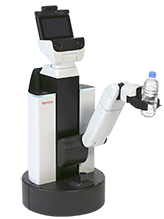
\includegraphics[width=0.25\textwidth]{images/toyota_hsr.png}
		\vspace{-10pt}
		\caption{Toyota HSR}
		\label{fig:toyotaHSR}
	\end{center}

	\vspace{-25pt}
	\begin{center}
		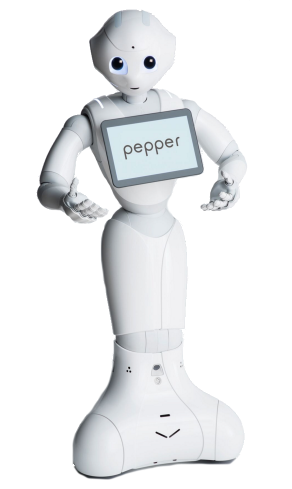
\includegraphics[width=0.20\textwidth]{images/softbank_pepper.png}
		\vspace{-10pt}
		\caption{Softbank / Aldebaran Pepper}
		\label{fig:softbank-pepper}
	\end{center}
\end{wrapfigure}
Each league points out to a different aspect of service robotics, reason for which they target specific abilities.


\subsection{Domestic Standard Platform League}
The \iterm{Domestic Standard Platform League}(DSPL) has as main goal to assist humans in a domestic environment, paying special attention to elderly people and people suffering of illness or disability. In consequence, the DSPL focuses on Ambient Intelligence, Computer Vision, Object Manipulation, Safe Indoor Navigation and Mapping, and Task Planning.

The robot to be used in the DSPL is the Toyota HSR, shown in Figure 1.1.

\subsection{Social Standard Platform League}
With a 180 degree turn in Human Robot Interaction, the \iterm{Social Standard Platform League}(SSPL) takes robots away from the traditional passive servant role, for now the robot is the one who will actively look for interaction. From a party waiter in a home environment to a hostess in a museum or shopping mall, in \iterm{SSPL} look for the next user who may require its services. Hence, this league focuses on Human-Robot Interaction, Natural Language Processing, People Detection and Recognition, Reactive Behaviors, and Safe Outdoor Navigation and Mapping.

The robot to be used in the SSPL is the Softbank/Aldebaran Pepper, shown in Figure 1.2.

\subsection{Open Platform League}
The \iterm{Open Platform League}(OPL) has the same modus operandi used since the fundation of RoboCup@Home till 2017 when Standard Platform Leagues were created. With no hardware constrains, OPL is the league for teams who want to test their own robot designs and configuration, as well as for old at-homers. In this league robots are tested to their limits without having in mind design restriction, although the scope is similar to the DSPL. 


%% %%%%%%%%%%%%%%%%%%%%%%%%%%%%%%%%%%%%%%%%%%%%%%%%%%%%%%%%%%%%%%%%%%%%%%%%%%%
%%
%%    author(s): RoboCupAtHome Technical Committee(s)
%%  description: Introduction - Competition
%%
%% %%%%%%%%%%%%%%%%%%%%%%%%%%%%%%%%%%%%%%%%%%%%%%%%%%%%%%%%%%%%%%%%%%%%%%%%%%%
\section{Competition}
The competition consists of 2 \emph{Stages} and the \iterm{Finals}. Each stage consists of a series of \iterm{Tests} that are being held in a daily life environment. The best teams from \iterm{Stage~I} advance to \iterm{Stage~II} which consists of more difficult tests. The competition ends with the \emph{Finals} where only the two highest ranked teams of each league compete to select the winner.

%% %%%%%%%%%%%%%%%%%%%%%%%%%%%%%%%%%%%%%%%%%%%%%%%%%%%%%%%%%%%%%%%%%%%%%%%%%%%
%%
%%    author(s): RoboCupAtHome Technical Committee(s)
%%  description: Introduction - Awards
%%
%% %%%%%%%%%%%%%%%%%%%%%%%%%%%%%%%%%%%%%%%%%%%%%%%%%%%%%%%%%%%%%%%%%%%%%%%%%%%
\section{Awards}
\label{sec:awards}
All the awards need to be approved by the RoboCup Federation (RCF). Based on RCF's decisions, some of them may not be given.

The RoboCup@Home league features the following \iterm{awards}.

\subsection{Winner of the competition}
\label{award:winner}
For each league, there will be a 1st, 2nd, and 3rd place award trophies (first and second place only when the number of teams is eight or less).

%
% As of 2017, the Execs have decided to remove the Innovation Award since
% is rarely given and its discussion is time consuming.
%
% \subsection{Innovation award}
% \label{award:innovation}
% To honour outstanding technical and scientific achievements as well as applicable solutions in the @Home league, a special \iterm{innovation award} may be given to one of the participating teams. Special attention is being paid to making usable robot components and technology available to the @Home community.
%
% The \iaterm{Executive Committee}{EC} members from the RoboCup@Home league nominate a set of candidates for the award. The \iaterm{Technical Committee}{TC} elects the winner. A TC member whose team is among the nominees is not allowed to vote.
%
% There is no innovation award in case no outstanding innovation and no nominees, respectively.


%
% As of 2017, the TC have decided to add an award for the best alternate HRI method
% to bypass speech recognition.
%
\subsection{Best Human-Robot Interface award}
\label{award:hri}
To honour outstanding Human-Robot Interfaces developed for interacting with robots in the @Home league, a special \iterm{Best HR Interface award} may be given to one of the participating teams. Special attention is being paid to making the interface open and available to the @Home community.

The \iaterm{Executive Committee}{EC} members from the RoboCup@Home league nominate a set of candidates for the award. The \iaterm{Technical Committee}{TC} elects the winner. A TC member whose team is among the nominees is not allowed to vote.

There is no Best HR Interface award in case no outstanding interface and no nominees, respectively.

\subsection{Best Poster}
\label{award:poster}
To foster scientific knowledge exchange and reward the teams' effort to present their contributions, as of 2017 all scientific posters of each League will be evaluated, having the chance of receiving the award for the \iterm{Best RoboCup @Home DSPL Poster}, the \iterm{Best RoboCup @Home OPL Poster}, or the \iterm{Best RoboCup @Home SSPL Poster}, respectively.

Candidate posters must present innovative and State-of-the-Art research within a field with direct application in RoboCup @Home in an appealing, easy-to-read way; demonstrating successful and clear results. In addition to be attractive and well-rated in the Poster Session (see~\refsec{sec:poster_teaser_session}), the explained research must have impact in the team's performance during the competition.

The \iaterm{Executive Committee}{EC} members from the RoboCup@Home league nominate a set of candidates for the award. The \iaterm{Technical Committee}{TC} elects the winner. A TC member whose team is among the nominees is not allowed to vote.

%
% As of 2013, the Execs have decided to remove the Innovation Award due to
% the lack of interest of the participants
%
% \subsection{Winner of the Technical Challenge}
% In parallel to the regular competition, the RoboCup@Home league features a \iterm{Technical Challenge}. The winner of the Technical Challenge is given a special \iterm{award for winning the Technical Challenge}.
%
% As with the innovation award, the award for winning the Technical Challenge is not given in case no team shows a \emph{sufficient performance}. The decision which team wins the Technical Challenge, and if the award is given at all, is conducted by the \iaterm{Technical Committee}{TC}.

\subsection{Skill Certificates}
\label{award:skill}
The @Home league features certificates for the robots best at a the skills below:
\begin{itemize}
   \item Navigation
   \item Manipulation
   \item Speech Recognition
   \item Person Recognition
  \end{itemize}

A team is given the certificate if it scored at least 75\% of the attainable points for that skill.
This is counted over all tests and challenges, so e.g.~if the robot scores manipulation points during the Help-me-Carry test to open the door, that will count for the Manipulation-certificate.
The certificate will only be handed out if the team is \emph{not} the overall winner of the competition.


\subsection{Open-source software award}
\label{award:oss}
Traditionally --since Nagoya 2017-- RoboCup@Home awards the best contribution to the community by means of open source software solutions. The software must be easy to read, properly documented, follow standard design patterns, be actively maintained, and meet IEEE software engineering metrics of scalability, portability, maintainability, fault tolerance, and robustness. In addition, the open sourced software must be made available as a framework-independent standalone library so it can be reused with any software architecture.

Candidates must send their application to the \iaterm{Technical Committee}{TC} at least one month before the competition by means of a short paper (max 4 pages) following the same format used for the \iterm{team description paper} (see~\refsec{rule:website_tdp}), including a brief explanation of the approach, comparison with State-of-the-Art techniques, statement of the used metrics and software design patterns, and the name of the teams and other collaborators that are also using the software being described.

The \iaterm{Technical Committee}{TC} members from the RoboCup@Home league nominate a set of candidates for the award. The \iaterm{Executive Committee}{EC} elects the winner. A EC/TC member whose team is among the nominees is not allowed to vote.


\subsection{Procter \& Gamble Dishwasher Challenge Award}
\label{award:skill}
\textit{Procter \& Gamble} gives an special award to the winner of the \textit{Procter \& Gamble Dishwasher Challenge}, typically to the team scoring higher in the challenge.
All teams can participate and compete for this award, regardless of whether they advanced to the Stage II or not, and get the award.

The award for winning the \textit{Procter \& Gamble Dishwasher Challenge} is not given in case no team shows a \emph{sufficient performance}. The decision on which team wins the \textit{Procter \& Gamble Dishwasher Challenge}, and if the award is given at all, is conducted by \textit{Procter \& Gamble}.


% Local Variables:
% TeX-master: "Rulebook"
% End:


\chapter{Concepts behind the competition}
\label{chap:concepts}
A set of conceptual key criteria builds the basis for the RoboCup@Home Competitions. These criteria are to be understood as a common agreement on the general concept of the competition. The concrete rules are listed in Chapter~\refsec{chap:rules}.

\section{Lean set of rules}
\label{concept:lean_set_of_rules}
To allow for different, general and transmissible approaches in the RoboCup@Home competitions, the rule set should be as lean as possible. Still, to avoid rule discussions during the competition itself, it should be very concrete leaving no room for diverse interpretation.

If, during a competition, there are any discrepancies or multiple interpretations, a decision will be made by the \iaterm{Technical Committee}{TC} and the referees on site.

\paragraph*{Note: } Once the test scoresheet has been signed or the scores has been published, the TC decision is irrevocable.

\section{Autonomy \& Mobility}
\label{concept:autonomy_and_mobility}
All robots participating in the RoboCup@Home competition have to be \emph{autonomous} and \emph{mobile}.

An aim of RoboCup@Home is to foster mobile autonomous service robotics and natural human-robot interaction. As a consequence humans are not allowed to directly (remote) control the robot. This also includes verbally remote controlling the robot.

Furthermore, the specific tasks must not be solved using \emph{open loop control}.

\section{Aiming for applications}
\label{concept:aiming_for_applications}
To foster advance in technology and to keep the competition interesting, the scenario and the tests will steadily increase in complexity. While in the beginning necessary abilities are being tested, tests will focus more and more on real applications with a rising level of uncertainty. Useful, robust, general, cost effective, and applicable solutions are rewarded in RoboCup@Home.

\section{\iterm{Social relevance}}
\label{concept:social_relevance}
The competition and the included tests should produce socially relevant results. The aim is to convince the public about the usefulness of autonomous robotic applications. This should be done by showing applications where robots directly help or assist humans in everyday life situations. Examples are: Personal robot assistant, guide robot for the blind, robot care for elderly people, etc. Such socially relevant results are rewarded in RoboCup@Home.

\section{Scientific value}
\label{concept:scientific_value}
RoboCup@Home should not only show what can be put into practice today, but should also present new approaches, even if they are not yet fully applicable or demand a very special configuration or setup. Therefore high scientific value of an approach is rewarded.

\section{Time constraints}
\label{concept:time_constraints}
Setup time as well as time for the accomplishment of the tests is very limited, to allow for many participating teams and tests, and to foster simple setup procedures.

\section{No standardized scenario}
\label{concept:no_standardized_scenario}
The \iterm{scenario} for the competition should be simple but effective, available world-wide and low in costs. As uncertainty is part of the concept, no standard scenario will be provided in the RoboCup@Home League. One can expect that the scenario will look typical for the country where the games are hosted.

The scenario is something that people encounter in daily life. It can be a home environment, such as a living room and a kitchen, but also an office space, supermarket, restaurant etc. The scenario should change from year to year, as long as the desired tests can still be executed.

Furthermore, tests may take place outside of the scenario, i.e., in an previously unknown environment like, for example, a public space nearby.

\section{Attractiveness}
\label{concept:attractiveness}
The competition should be attractive for the audience and the public. Therefore high attractiveness and originality of an approach should be rewarded.

\section{\iterm{Community}}
\label{concept:community}
Though having to compete against each other during the competition, the members of the RoboCup@Home league are expected to cooperate and exchange knowledge to advance technology together. The \iterm{RoboCup@Home mailing list} can be used to get in contact with other teams and to discuss league specific issues such as rule changes, proposals for new tests, etc.
% Since 2007 there is also the \iterm{RoboCup@Home Wiki} (see~\refsec{sec:at_home_wiki}) which serves as a central place to collect information relevant for the @Home league.
Every team is expected to share relevant technical, scientific (and team related) information there and in its \iterm{team description paper} (see~\refsec{rule:website_tdp}) through the team's website.

All teams are invited to submit papers on related research to the RoboCup Symposium which accompanies the annual RoboCup World Championship.

\section{Desired abilities}
\label{concept:desired_abilities}
This is a list of the current desired technical abilities which the tests in RoboCup@Home will focus on.

\begin{itemize}
\item Navigation in dynamic environments
\item Fast and easy calibration and setup \\ The ultimate goal is to have a robot up and running out of the box.
\item Object recognition
\item Object manipulation
\item Detection and Recognition of Humans
\item Natural human-robot interaction
\item Speech recognition
\item Gesture recognition
\item Robot applications \\ RoboCup@Home is aiming for applications of robots in daily life.
\item Ambient intelligence, e.g., communicating with surrounding devices, getting information from the internet etc.
\end{itemize}


% Local Variables:
% TeX-master: "Rulebook"
% End:


%% %%%%%%%%%%%%%%%%%%%%%%%%%%%%%%%%%%%%%%%%%%%%%%%%%%%%%%%%%%%%%%%%%%%%%%%%%%%
%%
%%          $Id: general_rules.tex 420 2013-04-08 15:30:35Z holz $
%%    author(s): RoboCupAtHome Technical Committee(s)
%%  description: description of the GENERAL RULES
%%
%% %%%%%%%%%%%%%%%%%%%%%%%%%%%%%%%%%%%%%%%%%%%%%%%%%%%%%%%%%%%%%%%%%%%%%%%%%%%
\chapter{General Rules \& Regulations}
\label{chap:rules}

These are the general rules and regulations for the competition in the RoboCup@Home league.
Every rule in this section can be considered to implicitly include the term \emph{\enquote{unless stated otherwise}}, meaning that additional or contrary rules in particular
test specifications have a higher priority than those mentioned herein in the general rules and regulations.

%%%%%%%%%%%%%%%%%%%%%%%%%%%%%%%%%%%%%%%%%%%%%%%%%%%%%%%%%
\section{Team Registration and Qualification}


\subsection{Registration and Qualification Process}
\label{rule:participation}

Each year there are four phases in the process toward participation:
\begin{enumerate}
	\item \iterm{Intention of Participation} (optional)
	\item \iterm{Preregistration}
	\item \iterm{Qualification} announcements
	\item Final \iterm{Registration} for qualified teams
\end{enumerate}
Positions 1 and 2 will be announced by a call on the \iterm{RoboCup@Home mailing list}. Preregistration requires a \iterm{team description paper}, a \Term{video}{qualification video} and a \Term{website}{Team Website}.

\subsection{Qualification Video}
As a proof of running hardware, each team has to provide a \iterm{qualification video} showing at least two from the following abilities (minimum requirement):
\begin{itemize}
	\item Human-Robot interaction
	\item Navigation (safe, indoors with obstacle avoidance).
	\item Object detection \& manipulation.
	\item People detection
	\item Speech recognition.
	\item speech synthesis (clear and loud).
\end{itemize}

Showing some of the following abilities is recommended:
\begin{itemize}
	\item Activity recognition
	\item Complex speech recognition
	\item Complex action planning
	\item Gesture recognition
\end{itemize}


Videos should be self-explicative and designed for a general audience, showing the  robot solving complex tasks. The minimum to qualify requires proving the robot is able to solve successfully at least one test of the current or last year's rulebook. For robots moving slowly, we suggest to speed-up videos. When doing so, please specify the speed factor being used (e.g.~2x, 5X, 10X). The same applies for slow motion scenes. Videos should not exceed the average time for a test (max.~\SI{10}{\minute}).

\subsection{Team Website}

The \iterm{Team Website} should be designed for a broader audience, and include scientific material (scientific papers, datasets, and documented open source code). Requirements are as follows:

\begin{enumerate}

	\item \textbf{Multimedia:}~As many photos and videos of the robot(s) as possible.

	\item \textbf{Language:}~The team website has to be in English. Other languages may be also available, but English must be default language.

	\item \textbf{Team:}~Comprehensive list of the team members including brief profiles.

	\item \textbf{RoboCup:}~Link to the league website and previous participation of the team in RoboCup.

	\item \textbf{Scientific approach:}~Include research lines, description of the approaches, and information on scientific achievements.

	\item \textbf{Publications:}~Relevant \iterm{publications} from 5 years up to date. Downloadable publications are scored higher during the qualification process.

	\item \textbf{Open source material:}~Blueprints, datasets, repositories or any kind of contribution to the league is highly scored during qualification process.
\end{enumerate}


\subsection{Team Description Paper}
\label{rule:website_tdp}
The \iaterm{team description paper}{TDP} is an 8-pages long scientific paper which must have a explained description of your main research, including the scientific contribution, goals, scope, and results.

Preferably, it should also contain the following:
\begin{itemize}
	\item the focus of research and the contributions in the respective fields,
	\item innovative technology (if any),
	\item re-usability of the system for other research groups
	\item applicability of the robot in the real world
	\item photo(s) of the robot(s)
\end{itemize}

~\\\noindent As addendum in the 9th page (after references) please include:
\begin{itemize}
	\item Team name
	\item Contact information
	\item Website url
	\item Team members' names
	\item photo(s) of the robot(s), unless included before.
	\item description of the hardware used
	\item Brief, compact list of \iterm{external devices} (See~\refsec{rule:robot_external_computing}), if any.
	\item Brief, compact list of 3rd party reused software packages (e.g.~ROS' \texttt{object\_recognition} should be listed, but not OpenCV).
	\item \textbf{[Open Platform League only]} Brief description of the hardware used by the robot(s).
\end{itemize}

~\\\noindent The TDP has to be in English, up to eight pages in length and formatted according to the guidelines of the RoboCup International Symposium without altering margins or spacing. It goes into detail about the technical and scientific approach.

Please notice that, during qualification process, TDP will be scored by its scientific value, novelty and contributions.


%% %%%%%%%%%%%%%%%%%%%%%%%%%%%%%%%%%%%%%%%
\subsection{Qualification}
\label{rule:qualification}

During the \iterm{qualification process} a selection will be made by the \iaterm{Organizing Committee}{OC} Taken into account and evaluated in this decision process are:
\begin{itemize}
	\item The content on the team website, scoring higher publications and open source resources;
	\item the number of abilities shown in the qualification video,
	\item the complexity of the tasks shown in the qualification video, and
	\item the scientific value, novelty and contributions in the \iterm{team description paper}. %, and
	% \item the information in the \iterm{RoboCup\char64Home Wiki} (added by the team).
\end{itemize}
(Additional) evaluation criteria are:
\begin{itemize}
	\item the performance in previous competitions,
	\item the relevant scientific contributions and publications, and
	\item the contributions to the RoboCup@Home league.
\end{itemize}

\paragraph{Important note to Standard Platform Leagues:} Only unmodified robots may compete in Standard Platform Leagues. Any \textit{slight} modification made to the robot found in the Qualification Material will automatically disqualify the team, for which registration to the international competition will not be possible  (See~\refsec{rule:spl-mods}).

% For getting considered in the evaluation, be sure to insert your team's name when adding information to the \iterm{RoboCup\char64Home Wiki}.


% Local Variables:
% TeX-master: "../Rulebook"
% End:


\section{Audience interaction}
Direct interaction with the audience is not a part of most challenges, though some explicitly require it in an effort to make robots step out of the laboratory.

Informing the audience however is important for the league.
\subsection{Vizbox}
\label{vizbox}

The objective of RoboCup is to \enquote{promote robotics and AI research, by offering a publicly appealing, but formidable challenge} \footnote{\url{http://robocup.org/objective}}.

Part of making RoboCup@Home appealing, is to show the audience what is going on, what the robots should do and what they are doing.

To this end, robots in RoboCup@Home are expected run the RoboCup@Home \href{https://github.com/LoyVanBeek/vizbox}{VizBox}\footnote{\url{https://github.com/LoyVanBeek/vizbox}}.

This is a web server to be run on a robot during a challenge. The page it serves can be displayed on a screen, visible to the audience, via a secondary computer in or around the arena, connected to the web server via the wireless network.

All robots are expected to run the \iterm{VizBox}; the audience expects to know what all the robots are doing and what each challenge entails.

The \iterm{VizBox}'s code is hosted \url{https://github.com/LoyVanBeek/vizbox}.
We want to show the audience a consistent presentation, so ideally, all teams run the same VizBox code.
Sharing your changes back in the form of a Pull Request is much appreciated so all teams can benefit.

The \iterm{VizBox} has the following visualization capabilities:
\begin{itemize}
	\item Images of what the robot sees or a visualization of the robot's world model, eg. camera images, it's map, anything to make clear what is going on to the audience.
	\item Show an outline of the current challenge and where the robot is in the story of the current challenge.
	\item Subtitles of what the robot and operator just said; their conversation
\end{itemize}

Additionally, the \iterm{VizBox} offers a way to \textbf{input} a text command to the robot, to bypass automatic speech recognition if need be.

The exact documentation is maintained in the repository of the \iterm{VizBox} itself.

%%%%%%%%%%%%%%%%%%%%%%%%%%%%%%%%%%%%%%%%%%%%%%%%%%%%%%%%%
\section{Scenario}
\label{sec:scenario}

The tests take place in the \iterm{RoboCup@Home arena}. Nonetheless, some tests can take place outside the arena, in a previously unknown public place. Rules in this section are related to the \iterm{RoboCup@Home arena} and its contents.

\subsection{RoboCup@Home arena}
The \iterm{RoboCup@Home arena} is a realistic home setting (apartment) consisting of inter-connected rooms.
The minimal configuration consists of
\begin{itemize}
	\item bedroom,
	\item dining room,
	\item living room, and
	\item kitchen.
\end{itemize}
Depending on the Local Organization, there may be multiple apartments which may be different to each other.
Robot must be prepared to perform any task in any arena, not the same arena every time.

The arena is decorated and dressed to resemble a typical apartment in the hosting country, including all necessities and decorations one can find in a normal house.
Please do note that what is considered as \enquote{normal} may greatly vary by culture and on the location where the RoboCup event is hosted.
Decorations include, but are not limited to: plants, mirrors, paintings, posters, plates, picture frames, wall clocks, candles with holders, and books.
For a description of objects, please refer to \refsec{rule:scenario_objects}

\subsection{Walls, doors and floor}
\label{rule:scenario_walls}

The indoor home setting will be surrounded by high and low \Term{walls}{Arena walls}.
These walls will be built up using standard fair construction material.

\begin{enumerate}
	\item \textbf{Walls:} Walls have a minimum height of \SI{60}{\centi\meter}. A maximum height is not specified, but must allow the audience to watch the competition.\\
	Walls are fixed and not to be modified during the competition (see~\refsec{rule:scenario_changes}).

	\item \textbf{Doors:} There will be at least two \Term{doors}{Arena doors}, an entrance and an exit, to be used as starting points for the robots (see~\refsec{rule:start_position}).
	% At least one of the entrances will be a door with a handle (not a knob).\
	Inside the arena rooms are connected by doors (at least one).
	All doors have handles, not knobs.
	Doors can be closed at any time, and it is expected that robots be able to open them.

	\item \textbf{Floor:} The floor of the arena as well as the doorways of the arena are even.
	That is, there will be no significant steps or even stairways.
	However, minor unevenness such as carpets, transitions in floor covering between different areas, and minor gaps (especially at doorways) can be expected.

	\item \textbf{Appearance:} Floor and walls are mainly uni-colored but can contain texture, e.g., a carpet on the floor, or a poster or picture on the wall.\\
	Although being unlikely at the moment, transparent elements are also possible.
\end{enumerate}


\subsection{Furniture}
\label{rule:scenario_furniture}
The arena will be equipped with typical objects (furniture) that are not specified in quantity and kind.

The minimal configuration consists of:
\begin{itemize}
	\item a bed,
	\item a couch,
	\item a small table,
	\item a small dinner table with two chairs,
	\item an open cupboard or small table with a television and remote control,
	\item a cupboard with drawers, and
	\item a bookcase or shelf with doors and some books inside
\end{itemize}

Likewise the arena's kitchen must have:
\begin{itemize}
	\item a dishwasher,
	\item a microwave,
	\item a sink, and
	\item a refrigerator in the kitchen (with some cans and plastic bottles inside).
\end{itemize}

A typical arena setup is shown in~\reffig{fig:scenario_arena}.

\begin{figure}[tbp]
	\centering
	\subfloat[Typical arena]{\label{fig:scenario_arena}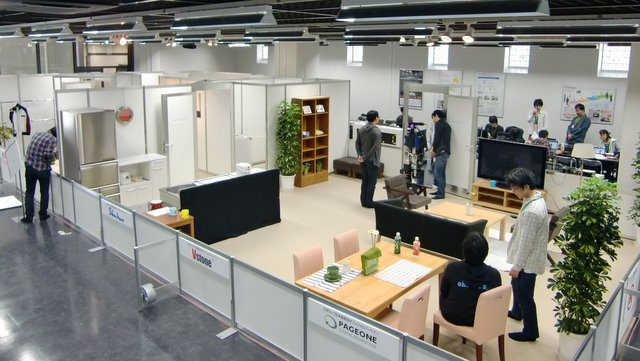
\includegraphics[height=46mm]{images/typical_arena.jpg}} ~
	\subfloat[Typical objects]{\label{fig:scenario_objects}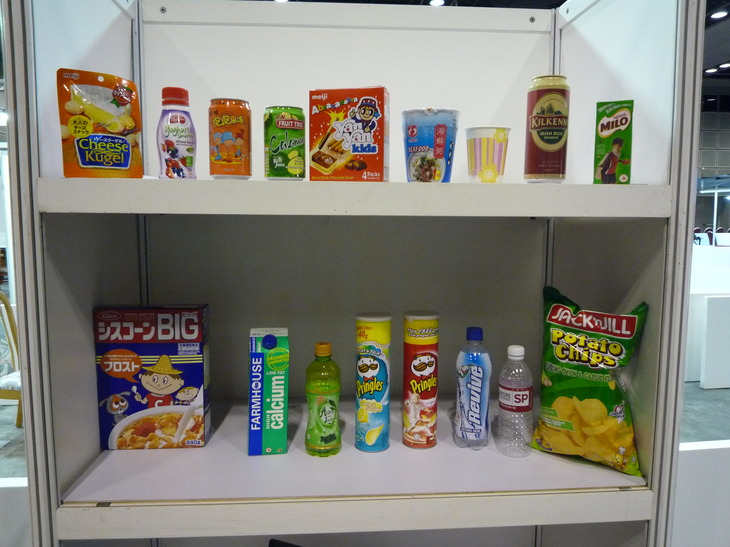
\includegraphics[height=46mm]{images/typical_objects.jpg}}
	\caption{Scenario examples: (a) a typical arena, and (b) typical objects.}
	\label{fig:arena}
\end{figure}


\subsubsection{Cupboard}
The cupboard can be any shelf-like furniture in which objects can be placed.
\begin{itemize}
	\item[\textbf{Doors:}] The cupboard may have doors.
	\item[\textbf{Drawers:}] The cupboard must have at least two drawers betweem 90cm and 120cm from floor level.
	\item[\textbf{Shelves:}] The minimum distance between shelf or layers is 30cm.
\end{itemize}

\subsubsection{Shelf}
A shelf, rack, or bookcase is required in RoboCup@Home.
The shelf can be any shelf-like furniture in which objects can be placed.
\begin{itemize}
	\item[\textbf{Doors:}] The shelf must have at least one door (preferrably a vertical one) covering up to one half of it.
	\item[\textbf{Drawers:}] The shelf must have no drawers.
	\item[\textbf{Shelves:}] The shelf must have 5 shelves or layers between 0.0m and 1.80m from the ground, with a minimum distance of 30cm between shelves or layers.
\end{itemize}

\subsubsection{Fridge}
Fridges must not be smaller than 120m. At least one powered and functioning fridge is required.


\subsection{Changes to the arena}
\label{rule:scenario_changes}

Since the robots should be able to function in the real world the scenario is not fixed and might change without further notice.
\begin{enumerate}
	\item \textbf{Major changes:}
	The arena is meant to be a simulated apartment.
	The furniture might be moved around between tests.
	This includes furniture that is a named location (see~\refsec{rule:scenario_names}).
	As in a normal home, furniture is not very likely to move from one room to another and is unlikely to be moved to the other side of a room.
	However, a couch or table may be rotated, moved to its side etc.
	Walls will stay in place and rooms will not change function.
	Passages might be blocked and cleared.
	One hour before a test slot begins no \iterm{major changes} will be made.
	This time will be shortened in the future.

	\item \textbf{Minor changes:} In contrast to major changes, \iterm{minor changes} like, for instance, slightly moved chairs cannot be avoided and may happen at any time (even during a test).
\end{enumerate}


%%%%%%%%%%%%%%%%%%%%%%%%%%%%%%%%%%%%%%%%%%%%%%%%%%%%%%%%%%%%%%%%%%
%
% Objects section.
%
% Revisited by Mauricio Matamoros for 2015
%
%%%%%%%%%%%%%%%%%%%%%%%%%%%%%%%%%%%%%%%%%%%%%%%%%%%%%%%%%%%%%%%%%%
\def\NumObjects{30\ }
\def\NumLocations{20\ }
\def\NumNames{20\ }

\subsection{Objects}
\label{rule:scenario_objects}
Some tests in the RoboCup@Home league involve recognizing and manipulating \iterm{objects}(See~\reffig{fig:scenario_objects}).
The TC will compile a list of at least \NumObjects objects for this purpose, assigning them official names.
Most objects are likely to be lightweight and easy to grasp with one hand.
Each object has assigned a category (e.g. an \textit{apple} and a \textit{banana} belong to the \textit{fruits} category).
Each \iterm{object category} has assigned a \iterm{predefined location} (e.g. an \textit{fruits} can be found in the \textit{kitchen table}).
Assignments are announced during setup days (See~\refsec{chap:setup_and_preparation}).
An exemplar of each object is provided before the competition for training.

There are two types of objects:

\begin{enumerate}
	\item \textbf{\iterm{Known objects}:} Objects previously known by the robot and that it can identify and manipulate.
	There are two kinds of known objects:
	\begin{enumerate}
		\item \textbf{\iterm{Regular objects}:} Objects with no noticeable difference among peers (e.g.~soda can, cereal box, cutlery, etc).
		\item \textbf{\iterm{Alike objects}:} Objects which are different one from another, but still considered by people to be the same (e.g.~apple, sandwich, cloth, etc.).
	\end{enumerate}

	\item \textbf{\iterm{Unknown objects}:} Any other object that is not known beforehand but can be grasped or handled.
\end{enumerate}

\subsection{List of Predefined Objects}
\label{rule:scenario_objects_list}
The minimal configuration consists of:
\begin{itemize}
	\item \textbf{\iterm{Tableware}:} Dish, bowl, cup (or mug), and napkin.
	\item \textbf{\iterm{Cutlery}:} Fork, knife, and spoon.
	\item \textbf{\iterm{Bags}:} Lightweight. With stiff, vertical handles.
	\item \textbf{\iterm{Trays}:} A transport object like a tray or basket. Intended for two-handed manipulation.
	\item \textbf{\iterm{Pourable}:} An object whose content can be poured (e.g. muesli, cereal, etc.).
	\item \textbf{\iterm{Heavy object}:} Weight between 1.0kg and 1.5kg).
	\item \textbf{\iterm{Tiny object}:} A lightweight object with no bigger than 5cm (e.g. paper, teabag, pen).
	\item \textbf{\iterm{Fragile object}:} An easy-to-break object, (e.g. chocolate egg).
	\item \textbf{\iterm{Amorphous object}:} An flexible object that may take an infinite number of shapes (e.g. cloth, magnetic puzzle, etc.).
\end{itemize}

\paragraph*{Important note:} It is not allowed to modify any of the objects provided for training.
Teams are not allowed to keep more than 5 the objects provided for training at a time nor retaining it for more than one hour.

\begin{figure}[H]
	\centering
	\subfloat[Bright-colored paper bags]{
		\label{fig:scenario_container_bag}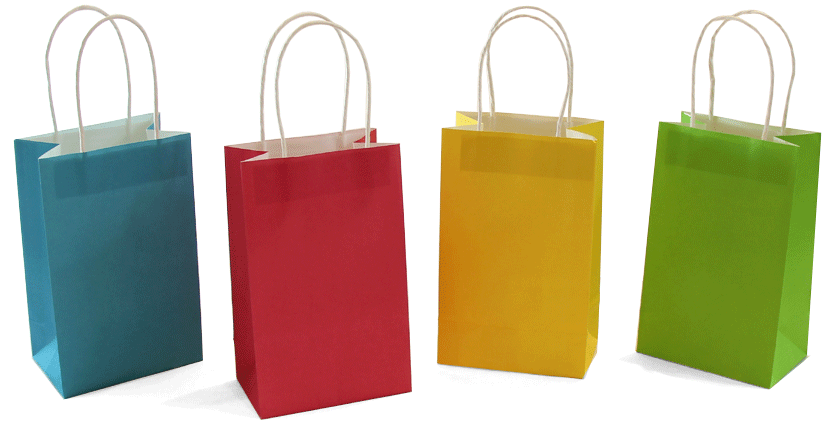
\includegraphics[width=0.33\textwidth]{images/container_paper_bag.png}}~
	\subfloat[Cereal bowls]{
		\label{fig:scenario_container_bowl}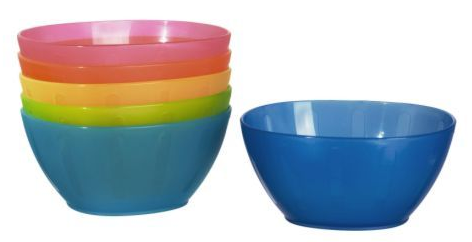
\includegraphics[width=0.33\textwidth]{images/container_bowl.png}}~
	\subfloat[Serving tray]{
		\label{fig:scenario_container_tray}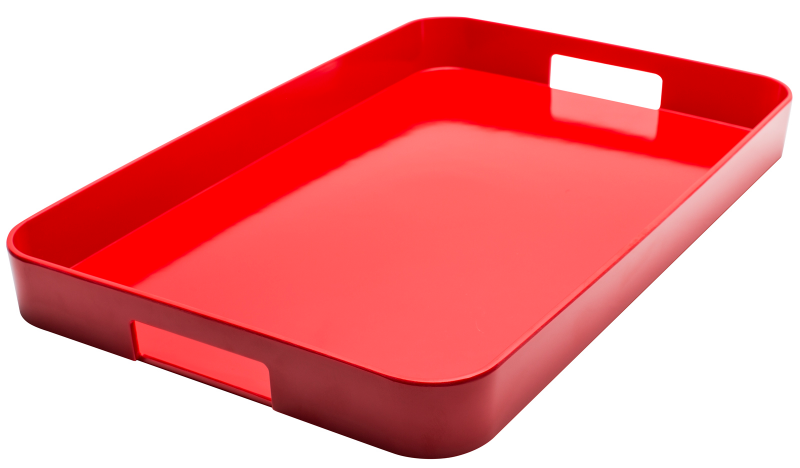
\includegraphics[width=0.33\textwidth]{images/container_tray.png}}
	\caption{Example of object containers}
	\label{fig:scenario_containers}
\end{figure}

\subsection{Attributes of Predefined Objects}
\label{rule:scenario_objects_attributes}
During the competition, objects can be requested based on their category \iterm{object category}, its physical attributes, or a combination of both.
Relevant attributes to be used are:
\begin{itemize}
	\item Color (e.g. red, blue, black with white dots, etc.).
	\item Relative estimated size (smallest, largest, big one, etc.).
	\item Relative estimated weight (lightest, heaviest).
	\item Relative position (left of, right most, etc.).
	\item Object description (is fragile, is container, can be poured, requires two hands, etc.).
\end{itemize}

\noindent\textbf{Remark:} Measurements are estimations and based on common sense. It is OK for robots to consider similar objects to be about the same size or weight.

%%%%%%%%%%%%%%%%%%%%%%%%%%%%%%%%%%%%%%%%%%%%%%%%%%%%%%%%%%%%%%%%%%
%
% Predefined locations section.
%
%%%%%%%%%%%%%%%%%%%%%%%%%%%%%%%%%%%%%%%%%%%%%%%%%%%%%%%%%%%%%%%%%%

\subsection{Predefined rooms and locations}
\label{rule:scenario_locations}
Some tests in the RoboCup@Home league involve \iterm{predefined locations} where people or objects can be found.
The TC will compile a list of predefined locations that may include furniture (e.g. bookshelf), decorations (e.g. plant, mirror), and doors.
Each \iterm{predefined location} has assigned a \iterm{location class} (e.g. an \textit{coach} and a \textit{arm chair} belong to the \textit{seat} class).
Room names, predefined locations, and location classes are announced during setup days (See~\refsec{chap:setup_and_preparation}).



\subsection{Predefined (person) names}\label{rule:scenario_names}
Some tests in the RoboCup@Home league involve memorizing a person name.
All people in the arena has an assigned \iterm{predefined name}.
The TC will compile a list of \NumNames \iterm{predefined names}.
The names are \SI{25}{\percent} male, \SI{25}{\percent} female, and \SI{50}{\percent} gender-neutral, taken from the list of most common used names in the United States.
Predefined names are announced during setup days (See~\refsec{chap:setup_and_preparation}).


\subsection{Wireless network}
\label{rule:scenario_wifi}

For wireless communication, an \iterm{arena network} is provided. The actual infrastructure depends on the local organization.
The organizers do NOT guarantee reliability and performance of wireless communication.
Teams required to start must do so regardless the availability of the network infrastructure.

The following rules apply:

\begin{itemize}
	\item Only the \iterm{arena network} can be used during tests.
	\item During the competitions, only the active team is allowed to use the \iterm{arena network}.
	\item The \iterm{arena network} provides one Virtual Local Area Networks (VLANs) per team.
	\item Each VLAN is most likely to have its own SSID/password.
	\item VLAN traffic is separated from any other team, routed to the team's network cable (team area).
	\item Each VLAN is also connected to the Internet.
\end{itemize}

\indent\textbf{Remark:} Teams broadcasting unauthorized (aka rogue) wireless networks will be disqualified from the competition, and have their devices confiscated by the OC.
This includes smartphones and concealed SSIDs.
It is advised to verify your devices.


% Local Variables:
% TeX-master: "../Rulebook"
% End:


%%%%%%%%%%%%%%%%%%%%%%%%%%%%%%%%%%%%%%%%%%%%%%%%%%%%%%%%%
\section{Robots}
\label{rule:robots}

\subsection{Number of robots}
\label{rule:robots_number}

\begin{enumerate}
	\item \textbf{Registration:} The maximum \term{number of robots} per team is \emph{two} (2).
	\item \textbf{Regular Tests:} Only one robot is allowed per test. For different tests different robots can be used.
	% \item \textbf{Open Demonstrations:} In the \iterm{Open Challenge} and the \iterm{Finals} both robots can be used simultaneously.
\end{enumerate}

\subsection{Appearance and safety}
\label{rule:robot_appearance}

Robots should have a nice product-like appearance, be safe to operate, and should not annoy people. The following rules apply to all robots and are part of the \iterm{Robot Inspection} test (see~\refsec{sec:robot_inspection}).
\begin{enumerate}
	\item \textbf{Cover:} The robot's internal hardware (electronics and cables) should be covered in an appealing way. The use of (visible) duct tape is strictly prohibited.
	\item \textbf{Loose cables:} Loose cables hanging out of the robot are not permitted.
	\item \textbf{Safety:} The robot must not have sharp edges or elements that might harm people.
	\item \textbf{Annoyance:} The robot must not be continuously making loud noises or use blinding lights.
	\item \textbf{Marks:} The robot may not exhibit any kind of artificial marks or patterns.
	\item \textbf{Driving:} To be safe, the robots should be careful when driving (obstacle avoidance is mandatory).
\end{enumerate}

\subsection{Standard Platform Leagues}
RoboCup@Home features two Standard Platform Leagues adhering to the rules listed above.

\subsubsection{Modifications}
\label{rule:spl-mods}
Standardized platforms allow teams to compete in equality of conditions by eliminating all hardware-dependent variables.
Therefore, modifications and alterations to the robots are strictly forbidden; including, but not limited to attaching, connecting, plugging, gluing, and taping components into and onto the robot, as well as modifying or altering the robot structure.
Voiding this rule leads to immediate disqualification from the competition and penalty for the team (see~\refsec{rule:extraordinary_penalties}).

During the \iterm{Robot Inspection} test (see~\refsec{sec:robot_inspection}), the TC will verify that the robot is in proper state for the competition; presenting no alterations and a neat condition.
EC and TC members may request re-inspection of a SPL robot at any time during the competition.

\textbf{Clothing, coloring, and stickers:} Robots are allowed to \enquote{wear} clothes, as well as have stickers (e.g., a sticker exhibiting the logo of an sponsor).
Painting the robot with another color or design is also allowed. 
However, artificial markers (e.g. bar codes, QR codes, OpenCV markers) are strictly forbidden. 
Teams should contact the robot providet before altering the robot's appearance.

% \subsubsection{Domestic Standard Platform League}
% The characteristics of the Toyota Human Support Robot are detailed below.

% \begin{itemize}
	% \item Aimed at human support tasks, elderly care et cetera
	% \item Omni-directional base, maximum speed 0.8km/h
	% \item 1 arm with multifunctional gripper through a vacuum pad. The wrist is equipped with a force-torque sensor. Capable of lifting 1.2kg.
	% \item RGB-D, stereo cameras and wide-angle camera
	% \item Display mounted in head, separate tablet interface
	% \item Access to cloud-based services
	% \item Equipped with a microphone array
	% \item Gravity compensated arm
	% \item Height-adjusting torso
% \end{itemize}
% 
% \subsubsection{Social Standard Platform League}
% The characteristics of the Softbank Robotics/Aldebaran Pepper are detailed below.
% 
% \begin{itemize}
	% \item Aimed at social interaction, public environments, explainable artificial intelligence
	% \item Omni-directional base, maximum speed 3km/h
	% \item 2 arms mostly intended for social gesturing.
	% \item 3D and 2 HD cameras
	% \item Equipped with a built-in tablet
	% \item Access to cloud-based services
	% \item Equipped with a 4-microphone array in the head
	% \item Emotion recognition by voice and images
	% \item Emotion engine to adapt it's attitude
% \end{itemize}

\subsection{Robot Specifications for the Open Platform League }
Robots competing in the RoboCup@Home Open Platform League must comply with security specifications in order to avoid causing any harm while operating in human environments.

\subsubsection{Size and weight of robots}
\label{rule:robots_size}

\begin{enumerate}
	\item \textbf{Dimensions:} The dimensions of a robot should not exceed the limits of an average door, which is \SI{200}{\centi\meter} by \SI{70}{\centi\meter} in most countries.\\
	The TC may allow the qualification and registration of larger robots, but due to the international character of the competition it cannot be guaranteed that the robots can actually enter the arena. In case of doubt, contact the local organization.
	\item \textbf{Weight:} There is no specific weight restriction. However, the weight of the robot and the pressure it exerts on the floor should not exceed local regulations for the construction of buildings which are used for living and/or offices in the country where the competitions is being held.
	\item \textbf{Transportation:} Team members are responsible for quickly moving the robot out of the arena.	If the robot cannot move by itself (for any reason), the team members must be able to transport the robot away with an easy and fast procedure.
\end{enumerate}



\subsubsection{Emergency stop button}
\label{rule:robots_emergency_button}

\begin{enumerate}
	\item \textbf{Accessibility and visibility:} Every robot has to provide an easily accessible and visible \iterm{emergency stop} button.
	\item \textbf{Color:} It must be coloured red, and be the only red button on the robot.
	The TC may ask the team to tape over or remove any other red button present in the robot.
	\item \textbf{Robot behavior:} When the \iterm{emergency stop} button is pressed, the robot and all its parts must stop moving immediately.
	\item \textbf{Inspection:} The emergency stop button is tested during the \iterm{Robot Inspection} test (see~\refsec{sec:robot_inspection}).
\end{enumerate}




\subsubsection{Start button}
\label{rule:start_button}

\begin{enumerate}
	\item \textbf{Requirements:} As stated in~\refsec{rule:start_signal}, teams that aren't able to carry out the default start signal (opening the door) have to provide a \iterm{start button} that can be used to start tests.
	Teams need to announce this to the TC before every test that involves a start signal, including \iterm{Robot Inspection}.

	\item \textbf{Definition:} The start button can be any \enquote{one-button procedure} that can be easily executed by a referee (e.g. releasing of the \iterm{emergency button} (\refsec{rule:robots_emergency_button}), a green button, or a software button in a Graphical User Interface).
	\item \textbf{Inspection:} The start button is tested during the the \iterm{Robot Inspection} test (see~\refsec{sec:robot_inspection}).
\end{enumerate}




% \subsubsection{Audio output plug}
% \label{rule:roobt_audio_out}

% \begin{enumerate}
% 	\item \textbf{Mandatory plug:} Either the robot or some external device connected to it \emph{must} have a \iterm{speaker output plug}. It is used to connect the robot to the sound system so that the audience and the referees can hear and follow the robot's speech output.
% 	\item \textbf{Inspection:} The output plug needs to be presented to the TC during the \iterm{Robot Inspection} test (see~\refsec{sec:robot_inspection}).
% 	\item \textbf{Audio during tests:} Audio (and speech) output of the robot during a test have to be understood at least by the referees and the operators.
% 	\begin{compactitem}
% 		\item It is the responsibility of the teams to plug in the transmitter before a test, to check the sound system, and to hand over the transmitter to next team.
% 		\item Do not rely on the sound system! For fail-safe operation and interacting with operators make sure that the sound system is not needed, e.g., by having additional speakers directly on the robot.
% \end{compactitem}
% \end{enumerate}




\subsubsection{Appearance}
\label{rule:robots_appearance}
Open Platform Robots should have a neat appearance that resembles more a safe and finished product than an early stage prototype, paying special attention in completely cover the robot's internal hardware (electronics and cables) in an appealing way.
% However, teams must keep in mind that no artificial markers are allowed when personalizing the appearance or a robot. This includes, but is not limited to bar codes, QR codes, OpenCV markers, fluorescent and phosphorescent colors, and reflective stickers.
Although covering the robot's internal hardware with a T-Shirt is not forbidden (for now) it is strongly unadvised.



% Local Variables:
% TeX-master: "../Rulebook"
% End:


% %% %%%%%%%%%%%%%%%%%%%%%%%%%%%%%%%%%%%%%%%%%%%%%%%%%%%%%%%%%
% 
% External Devices
% 
% %% %%%%%%%%%%%%%%%%%%%%%%%%%%%%%%%%%%%%%%%%%%%%%%%%%%%%%%%%%

\section{External devices}
\label{rule:robot_external_devices}
Everything which is not part of the robot is considered an \iterm{external device}.
All external devices must be authorized by the \iaterm{Technical Committee}{TC} during the \iterm{Robot Inspection} test (see~\refsec{sec:robot_inspection}).
The \iaterm{Technical Committee}{TC} specifies whether an external device can be used freely, under referee supervision, and its impact on scoring.
In general, external devices must be removed quickly after the test.
	
\noindent \textbf{Remark:} The use of \iterm{wireless devices} is strictly prohibited. \iterm{External microphones}, hand microphones, and headsets are not allowed in OPL and it use is discouraged in DSPL and SSPL.

\subsection{On-site external computing}
Computing resources that are not physical attached to the robot are considered \iterm{external computing resources}.
The use of up to 5 external computing resources is allowed, but only through the arena network (see \refsec{rule:scenario_wifi}) and with the previous approval of the \iaterm{Technical Committee}{TC}.
Teams must announce the use of any external computing resource at least 1 month before the competition to the \iaterm{Technical Committee}{TC}.

External Computing Devices must be placed in the \iaterm{\textbf{E}xternal \textbf{C}omputing \textbf{R}esource \textbf{A}rea}{ECRA} which is announced by the \iaterm{Technical Committee}{TC} during setup days.
A switch connected to the arena wireless network will be available to teams in the ECRA.
It is strictly forbidden to connect any kind of device or peripheral (e.g. screens, mouses, keyboards, etc.) to the computers in the ECRA during the competition.

A maximum of two laptops and two people from different teams is allowed at any time in the ECRA.
Teams using laptops as External Computing Devices must remove the device immediately after the test.
Once a test has started, all people must stay at least 1 meter from the ECRA.
Interacting with computers in the ECRA after the Referee has given the start signal will cause the immediate disqualification of the team.

\noindent \textbf{Remark:} Robot operation must be able to operate safely when \iterm{external computing resources} are unavailable.



% On-line devices
\subsection{On-line external computing}
\label{rule:robot_external_computing_online}
Robots are allowed to use \enquote{Cloud services}, \enquote{Internet API's}, and any other type of \iterm{external computing resource}.
Same restrictions for on-site external computing resources apply.

\noindent \textbf{Remark:} The competition organization doesn't guarantee or take any responsibility regarding the availability or reliability of neither the network nor Internet connection.
Teams' use of external computing resources is at their own risk.



% DSPL laptop
\subsection{Official Standard Laptop for DSPL}
\label{rule:osl_dspl}

In the Domestic Standard Platform League, teams may use the \iaterm{Official Standard Laptop}{OSL} connected to the Toyota HSR via Ethernet cable, safely located in the TOYOTA HSR \iterm{Mounting Bracket} provided by TOYOTA for this purpose.

\subsubsection{Technical Specifications}
The technical specifications for the Official Standard Laptop in the Domestic Standard Platform League are the following:


 \begin{itemize}
  \item \textbf{Brand and model:} DELL Alienware 15 or 17
  \item \textbf{CPU:} Core-i7 series
  \item \textbf{RAM:} 16GB or 32GB
  \item \textbf{GPU:} NVIDIA GeForce GTX 1070 or 1080
  \item \textbf{Storage:} Unrestricted.
\end{itemize}

No other brands or models will be accepted. There are no constrains regarding the software installed in the OSL but no additional hardware is allowed.

The referees, Technical Committee, and Organizing Committee members may run random checks anytime during the competition prior to the test to verify that the laptop in the TOYOTA HSR \iterm{Mounting Bracket} has no additional hardware plugged in, and matches the authorized specifications.


% Local Variables:
% TeX-master: "../Rulebook"
% End:


%%%%%%%%%%%%%%%%%%%%%%%%%%%%%%%%%%%%%%%%%%%%%%%%%%%%%%%%%
\section{Organization of the competition}
\label{sec:procedure_during_competition}

\subsection{Stage system}\label{rule:stages}

The competition features a \iterm{stage system}. It is organized in two stages each consisting of a number of specific tasks. It ends with the \iterm{Finals}.

Each \iaterm{stage} comprehends a set of tasks grouped in two thematic scenarios.
% \iaterm{House Cleaner} and \iaterm{Party Host}.
The \iaterm{House Holder} scenario features tasks related to cleaning, organizing, and giving maintenance; while the \iaterm{Party Host} scenario focuses in attending guests needs and providing general assistance during a party.

\begin{enumerate}
	\item \textbf{Robot Inspection:} For security, robots are inspected during setup days. A robot must pass \iterm{Robot Inspection} test (see~\refsec{sec:robot_inspection}) in order to compete.

	\item \textbf{Stage~I:} The first days of the competition called \iterm{Stage~I}.
	All qualified teams can participate in \iterm{Stage~I}.
	The same task can be performed multiple times (See~\refsec{rule:score_system}).

	\item \textbf{Stage~II:} The best \emph{50\% of teams}\footnotemark (after Stage~I) advance to \iterm{Stage~II}.
	Here, tasks require more complex abilities or combinations of abilities.\\
	\footnotetext{If the total number of teams is less than 12, up to 6 teams may advance to Stage~II}
	The \iterm{Open Challenge} is the open demonstration in Stage~II.

	\item \textbf{Final demonstration:} The best \emph{two teams} of each league, the ones with the highest score after Stage~II, advance to the final round.
	The final round features only a single task integrating all tested abilities.
	In order to participate in the Finals, a team must have solved at least one task of the Stage~II.
\end{enumerate}

In case of having no considerable score deviation between a team advancing to the next stage and a team dropping out, the TC may announce additional teams advancing to the next stage.


%%%%%%%%%%%%%%%%%%%%%%%%%%%%%%%%%%%%%%%%%%%%%%%%%%%%%%%%%
\subsection{Schedule}
\label{rule:schedule}

\begin{enumerate}
	\item \textbf{Thematic scenario blocks:} Each \iterm{thematic scenario} or \iterm{theme} is split in two \iterm{blocks}.
	At least two blocks are scheduled per day, having each block an assigned theme and lasting no less than two hours.
	The \iaterm{Organizing Committee}{OC} announces the schedule during the setup days (see Table \ref{tbl:schedule}).

	\item \textbf{Slots:} The \iaterm{Organizing Committee}{OC} assigns at least two \iterm{test slots} of 5 minutes to each team in each block.
	A team can solve any task during its test slot.
	Remaining block time can be used to assign additional testing slots to interested teams.
	Testing slots are randomly assigned to teams in each block.

	\item \textbf{Tests:} Teams must inform the OC in advance which task(s) will try to solve.
	Only one task can be attempted per test slot.

	\item \textbf{Participation is default:} Teams have to indicate to the \iaterm{Organizing Committee}{OC} when they are \emph{skipping} a test slot. Without such indication, they may receive a penalty when not attending (see~\refsec{rule:not_attending}).
\end{enumerate}

% Please add the following required packages to your document preamble:
% \usepackage[table,xcdraw]{xcolor}
% If you use beamer only pass "xcolor=table" option, i.e. \documentclass[xcolor=table]{beamer}
\begin{table}[h]
	\centering\small
	\newcommand{\teams}[3]{%
		\tiny
		\begin{tabular}{c}%
			\textit{Test slot 1, team $#1$}\\
			\textit{Test slot 2, team $#2$}\\
			$\vdots$\\
			\textit{Test slot $n$, team $#3$}\\
		\end{tabular}
	}
	\newcommand{\wcell}[2]{%
		\parbox[c]{2.5cm}{%
			\vspace{#1}%
			\centering%
			#2%
			\vspace{#1}%
		}%
	}
	\newcommand{\cell}[1]{\wcell{0.2\baselineskip}{#1}}


	\begin{tabular}{
		>{\centering\arraybackslash}m{2.5cm}|%
		>{\columncolor[HTML]{9AFF99}}c |%
		>{\columncolor[HTML]{9AFF99}}c |%
		>{\columncolor[HTML]{CBCEFB}}c |%
		>{\columncolor[HTML]{CBCEFB}}c |%
	}
	\multicolumn{1}{ c }{}
		& \multicolumn{1}{ c }{\cellcolor{white} Day 1 }
		& \multicolumn{1}{ c }{\cellcolor{white} Day 2 }
		& \multicolumn{1}{ c }{\cellcolor{white} Day 3 }
		& \multicolumn{1}{ c }{\cellcolor{white} Day 4 }
		\\\cline{2-5}
	\cell{Block 1\\\footnotesize(9:00 - 12:00)}
		& \cell{House Holder\\\teams{i}{j}{i}}
		& \cell{Party Host\\\teams{k}{i}{k}}
		& \cell{House Holder\\\teams{i}{j}{i}}
		& \cell{Party Host\\\teams{j}{k}{j}}\\\cline{2-5}

	\multicolumn{1}{ c }{}
		& \multicolumn{4}{ c }{\wcell{0.5\baselineskip}{\color{gray}Lunch}}\\\cline{2-5}

	\cell{Block 2\\\footnotesize(9:00 - 12:00)}
		& \cell{House Holder\\\teams{i}{k}{i}}
		& \cell{Party Host\\\teams{k}{j}{k}}
		& \cell{Party Host\\\teams{i}{i}{k}}
		& \cell{House Holder\\\teams{k}{j}{j}}\\\cline{2-5}

	\multicolumn{1}{ c }{}
		& \multicolumn{2}{ c }{\wcell{0.5\baselineskip}{\color[HTML]{029734}Stage 1}}
		& \multicolumn{2}{ c }{\wcell{0.5\baselineskip}{\color[HTML]{6668e5}Stage 2}}\\
	\end{tabular}

	\caption{Example schedule.
		Each team has assigned at least two test slots in every block.
		At least two blocks are scheduled per day with an assigned theme.
		A team can choose a different task in each test, meaning at least 4 different tests per stage.
	}
	\label{tbl:schedule}
\end{table}


\subsection{Score system}
\label{rule:score_system}
Each task has a main objective and a set of scoring bonuses.
To score in a test, a team must successfully accomplish the main objective of the task; bonuses are not considered otherwise.
Overall scoring is calculated as the sum of the maximum score obtained in each ability.

The \iaterm{score system} has the following constrains
\begin{enumerate}
	\item \textbf{Stage~I:} The maximum total score per task in \iterm{Stage~I} is \scoring{1000 points}.
	
	\item \textbf{Stage~II:} The maximum total score per task in \iterm{Stage~I} is \scoring{2000 points}.

	\item \textbf{\iterm{Finals}:} Final score is normalized and a special evaluation is used.

	\item \textbf{Minimum score:} The minimum total score per test in \iterm{Stage~I} and \iterm{Stage~II} is \scoring{0 points}.
	Teams cannot receive negative points.

	\item \textbf{Penalties:} An exception to \emph{minimum score} rule are penalties.
	Both penalties for not attending (see~\refsec{rule:not_attending}) and extraordinary penalties (see~\refsec{rule:extraordinary_penalties}) can cause a total negative score.
\end{enumerate}




% Local Variables:
% TeX-master: "../Rulebook"
% End:


%%%%%%%%%%%%%%%%%%%%%%%%%%%%%%%%%%%%%%%%%%%%%%%%%%%%%%%%%
\section{Procedure during Tests}

\subsection{Safety First!}
\label{rule:safetyfirst}
\begin{enumerate}
	\item \textbf{Emergency Stop:} At any time when operating the robot inside and outside the scenario the owners have to stop the robot immediately if there is a remote possibility of dangerous behavior towards people and/or objects.
	\item \textbf{Stopping on request:} If a referee, member of the Technical or Organizational committee, an Executive or Trustee of the federation tells the team to stop the robot, there will be no discussion and the robot has to be stopped \emph{immediately}.
	\item \textbf{Penalties:} If the team does not comply, the team and its members will be excluded from the ongoing competition immediately by a decision of the RoboCup@Home \iaterm{Technical Committee}{TC}. 	Furthermore, the team and its members may be banned from future competitions for a period not less than a year by a decision of the RoboCup Federation Trustee Board.
\end{enumerate}

\subsection{Maximum number of team members}
\label{rule:number_of_people}
\begin{enumerate}
	\item \textbf{Regular Tests:} During a regular test, the maximum number of team members allowed inside the arena is \emph{one} (1).
	Exceptions are tests that explicitly require volunteer assistance.
	\item \textbf{Setup:} During the setup of a test, the number of team members inside the arena is not limited.
	\item \textbf{Moderation:} During a regular test, one team member \emph{must} be available to host and comment the test (see~\refsec{rule:moderator}).
\end{enumerate}

\subsection{Fair play}
\label{rule:fairplay}
\iterm{Fair Play} and cooperative behavior is expected from all teams during the entire competition, in particular:
\begin{itemize}
	\item while evaluating other teams,
	\item while refereeing, and
	\item when having to interact with other teams' robots.
\end{itemize}
This also includes:
\begin{itemize}
	\item not trying to cheat (e.g.~pretending autonomous behavior where there is none),
	\item not trying to exploit the rules (e.g.~not trying to solve the task but trying to score), and
	\item not trying to make other robots fail on purpose.
	\item not modifying robots in standard platforms.
\end{itemize}
Disregard of this rule can lead to penalties in the form of negative scores, disqualification for a test, or even for the entire competition.

\subsection{Expected Robot's Behavior}
Unless stated otherwise, it is expected that the robot always behave and react in the same way a polite and friendly human being would do.
This applies also to how robots try solve the assigned task
As rule of thumb, one may ask any non-scientist how she would solve the task.

Please consider that average users will not know the specific procedure to operate a robot.
Hence, interaction should be as with any other human being.


\subsection{Robot Autonomy and Remote Control}
\begin{enumerate}
	\item \textbf{No touching:} During a test, the participants are not allowed to make contact with the robot(s), unless it is in a \enquote{natural} way and required by the task.

	\item \textbf{Natural interaction:} The only allowed means to interact with the robot(s) are gestures and speech.

	\item \textbf{Natural commands:} Anything that resembles direct control is forbidden.

	\item \textbf{Remote Control:} Remotely controlling the robot(s) is strictly prohibited.
	This also includes pressing buttons, or influencing sensors on purpose.

	\item \textbf{Penalties:} Disregard of these rules will lead to disqualification for a test or for the entire competition.
\end{enumerate}



\subsection{Collisions}
\begin{enumerate}
	\item \textbf{\iterm{Touching}:} Gently \emph{touching} objects is tolerated but unadvised.
	However, robots are not allowed to crash with something.
	The \enquote{safety first} rule (\refsec{rule:safetyfirst}) overrides any other rule.

	\item \textbf{\iterm{Major collisions}:} If a robot crushes into something during a test, the robot is immediately stopped.	Additional penalties may apply.

	\item \textbf{\iterm{Functional touching}:} Robots are allowed to apply pressure on objects, push away furniture and, in general, interact with the environment using structural parts other than their manipulators.
	This is known as \iaterm{functional touching}.
	However, the robot must clearly announce the collision-like interaction and kindly request not being stopped.\\
	\textbf{Remark: } Referees can (and will) immediately stop a robot in case or suspicion of \emph{dangerous} behavior.
	
	\item \textbf{Robot-Robot avoidance:} If two robots encounter each other, they both have to actively try to avoid the other robot.
	\begin{enumerate}
		\item A robot which is not going for a different route within a reasonable amount of time (e.g., \SI{30}{\second}) is removed.
		\item A non-moving robot blocking the path of another robot for longer than a reasonable amount of time (e.g., \SI{30}{\second}) is removed.
	\end{enumerate}
\end{enumerate}



\subsection{Removal of robots}
\label{rule:robot_removal}
Robots not obeying the rules are stopped and removed from the arena.
\begin{enumerate}
	\item It is the decision of the referees and the TC member monitoring the test if and when to remove a robot.
	\item When told to do so by the referees or the TC member monitoring the test, the team has to immediately stop the robot, and remove it from the arena without disturbing the ongoing test.
\end{enumerate}


\subsection{Start signal}
\label{rule:start_signal}
The default \iterm{start signal} (unless stated otherwise) is \iterm{door opening}.
Other start signals are allowed but must be authorized by the \iaterm{Technical Committee}{TC} during the Robot Inspection (see~\refsec{sec:robot_inspection}).

\begin{enumerate}
	\item \textbf{Door opening:} The robot is waiting behind the door, outside the arena and accompanied by a team member.
	The test starts when a referee (not a team member) opens the door.

	\item \textbf{Start button:} If the robot is not able to automatically start after the door is open, the team may start the robot using a start button.
	\begin{enumerate}
		\item Using a start button needs to be announced to the referees. It is the responsibility of the team to do so before the test starts.
		\item Any single-key-press procedure is allowed. Typing commands is strictly forbidden.
		\item There may be penalties for using a start button in some tests
	\end{enumerate}

	\item \textbf{QR Codes:} If the robot is not able to automatically start after the door is open, the team may start the robot by showing it a QR code.

	\item \textbf{Verbal instructions:} If the robot is not able to automatically start after the door is open, the team may start the robot using a verbal command.

	\item \textbf{Ad-hoc start signal:} Other means of triggering robot to action must be approved by the \iaterm{Technical Committee}{TC} during the Robot Inspection (see~\refsec{sec:robot_inspection}).
\end{enumerate}


\subsection{Entering and leaving the arena}
\label{rule:start_position}
\begin{enumerate}
	\item \textbf{Start position:} Unless stated otherwise, the robot starts outside of the arena.
	\item \textbf{Entering:} The robot has to autonomously enter the arena.
	\item \textbf{Success:} The robot is said to \emph{have entered} when the door used to enter can be closed again, and the robot is not blocking the passage.
\end{enumerate}



\subsection{Gestures}
\label{rule:gestures}
Hand gestures may be used to control the robot in the following way:
\begin{enumerate}
	\item \textbf{Definition:} The teams define the hand gestures by themselves.

	\item \textbf{Approval:} Gestures need to be approved by the referees and TC member monitoring the test. Gestures should not involve more than the movement of both arms. This includes e.g.~expressions of sign language or pointing gestures.

	\item \textbf{Instructing operators:} It is the responsibility of the team to instruct operators.
	\begin{enumerate}
		\item The team may only instruct the operator when told to so by a referee.
		\item The team may only instruct the operator in the presence of a referee.
		\item The team may only instruct the robot for as long as allowed by the referee.
		\item When the robot has to instruct the operator, it is the robot that instructs the operator and \emph{not} the team. The team is not allowed to additionally guide the operator, e.g., tell the operator to come closer, speak louder, or to repeat a command.
		\item The robot is allows to instruct the operator at any time.
	\end{enumerate}

	\item \textbf{Receiving gestures:} Unless stated otherwise, it is not allowed to use a speech command to set the robot into a special mode for receiving gestures.
\end{enumerate}



\subsection{Referees}
\label{rule:referees}
All tests are monitored by a referee and one member of the \iaterm{Technical Committee}{TC}.
The following rules apply:

\begin{enumerate}
	\item \textbf{Selection:}
	\begin{itemize}
		\item Referees are chosen by EC/TC/OC.
		\item Referees are announced together with the schedule for the test slot.
	\end{itemize}

	\item \textbf{Not showing up:} Not showing up for refereeing (on time) will result in a penalty (see~\refsec{rule:extraordinary_penalties}).

	\item \textbf{TC monitoring:} A TC member acts as main referee.

	\item \textbf{Referee instructions:} Right before each test, referee instructions are conducted by the TC.
	The referees for all slots need to be present at the arena where the referee instructions are taking place.
	When and where referee instructions are taking place is announced together with the schedule for the slots.
\end{enumerate}


\subsection{Operators}
\label{rule:operator}
Unless stated otherwise, robots are operated by the referee or by a person selected by the referee.
If the robot fails to understand the default operator, the team may request the use of a custom operator.
Penalty may apply when using a custom operator.


\subsection{Moderator}
\label{rule:moderator}
The LOC is responsible of organizing test moderation in the local language.
The OC may request the participating teams to provide a team member for moderation.
Candidates have to be fluent in the moderation language (default is English).

\noindent\textbf{Responsibilities:} The moderators have to:
\begin{compactitem}
	\item Do \textbf{NOT interfere} with the performance
	\item Explain the tasks being performed
	\item Comment on the performance of the competitor
	\item Follow the instructions of the referee.
\end{compactitem}

\noindent \textbf{Not showing up:} Not showing up for moderation (on time) will result in a penalty (see~\refsec{rule:extraordinary_penalties}).


\subsection{Time limits}
\label{rule:time_limits}
\begin{enumerate}
	\item \textbf{Stage~I:} Unless stated otherwise, the time limit for each test in \iterm{Stage~I} is \timing{5 minutes}.

	\item \textbf{Stage~II:} Unless stated otherwise, the time limit for each test in \iterm{Stage~II} is \timing{10 minutes}.

	\item \textbf{Inactivity:} Robots are not allowed to stand still or get stuck into endless loops.
	A robot not progressing in the task execution (and obviously not trying to), is consider as inactive.
	Robots must be removed after 30 seconds of inactivity.

	\item \textbf{Requesting time:} A robot (not the team) can request referees to make exception from the 30-seconds inactivity time limit.
	In its request, the robot has to clearly state for how long it will be performing a time-consuming process (e.g. 60~seconds).
	This time cannot exceed 3 minutes and cannot be used more than once per test.

	\item \textbf{Setup time:} Unless stated otherwise, there is no setup time.
	Robots need to be ready to enter the arena no later than one minute after the door has been closed to the former team.

	\item \textbf{Time-up:} When the time is up, the team has to immediately remove their robot(s) from the arena.
	No more additional score will be giving.

	\item \textbf{Show must go on:} On special cases, the referee may let the robot continue the test for demonstration purposes, but no additional points will be scored.
\end{enumerate}



\subsection{Restart}
\label{rule:restart}
Some tasks allow a single restart, a procedure in which the team is allowed to quickly fix any issue with the robot.
Restarts can be requested only when the test slot permits it, and when the amount of remaining time is greater than 50\% of the total.
The procedure is as follows:

\begin{enumerate}
	\item The team request a restart.
	\item The robot is taken to the initial position (e.g. outside the arena) and gets fixed.
	\item When the robot is ready, the team informs the referee.
\end{enumerate}

The following rules apply:
\begin{enumerate}
	\item \textbf{Number of restarts:} When allowed, the maximum number of restarts is one (1).

	\item \textbf{Early request:} Restart is \textbf{NOT} allowed after the first 50\% of the alloted time has elapsed.

	\item \textbf{Time:} The timer is neither restarted nor stopped. 

	\item \textbf{One-minute Setup} The team has 1 minute to fix the robot counting when the referee announces th restart.
	If the robot is not ready, the test is considered finished.

	\item \textbf{Scoring:} If the score of the second attempt is lower than the score of the first one, the average score of first and second run is taken.
	
	\end{enumerate}

% Local Variables:
% TeX-master: "../Rulebook"
% End:

\section[Deus ex Machina]{Deus ex Machina: Bypassing features with human help \\ \small Because the show must go on}
\label{rule:continue}
Robots can't score unless they accomplish the main goal of a task.
However, in many real-life situations, a minor malfunction may prevent the robot from accomplishing a task.
To prevent this situation, while fostering awareness and human-robot interaction, robots are allowed to request human assistance during a test.

\subsection{Procedure}
\label{rule:continue_procedure}
The procedure to request human assistance while solving a task is as follows:

\begin{enumerate}
	\item \textbf{Request help:} The robot must indicate loud and clear that it requires human assistance. It must be clearly stated:
	\begin{compactitem}
		\item The nature of the assistance
		\item The particular goal or desired result
		\item How the action must be carried out (when necessary)
		\item Details about how to interact with the robot (when necessary)
	\end{compactitem}

	\item \textbf{Supervise:} The robot must be aware of the human's actions, being able to tell when the requested action has been completed, as well as guiding the human assistant (if necessary) during the process.

	\item \textbf{Acknowledge:} The robot must politely thank the human for the assistance provided.
\end{enumerate}

\subsection*{Example}
\label{rule:continue_example}
In this example the robot has to clean the table but is unable to grasp the spoon. 
\begin{itemize}[noitemsep]
	\small
	\item[\textcolor{gray}{R:}] \texttt{I am sorry but the spoon is too small for me to take.\\
	Could you please help me with it?\\
	Please say "robot yes" or "robot no" to confirm.}
	\item[\textcolor{gray}{H:}] \textit{Robot, yes!}
	\item[\textcolor{gray}{R:}] \texttt{Thank you! Please follow my instructions.\\
	Please take the purple spoon from the table. It is on my left.}
	\item[\textcolor{gray}{H:}] (Referee takes green fork)
	\item[\textcolor{gray}{R:}] \texttt{You took the wrong object.\\
	Please take the purple spoon from the table. It is on my left.}
	\item[\textcolor{gray}{H:}] (Referee takes purple spoon)
	\item[\textcolor{gray}{R:}] \texttt{I saw you took the spoon.\\
	Would you be so kind of following me to the kitchen?\\
	Please keep the spoon visible in front of you so I can track you. Thank you!}
	\item[\textcolor{gray}{R:}] \texttt{You can stop following me now.\\
	As you can see, the dishwasher is already open.\\
	Please place the spoon in the gray basket on the lower tray.}
	\item[\textcolor{gray}{R:}] \texttt{Lovely! Thanks for your help human.\\
	I'll let you know if I need further assistance.}
\end{itemize}



\subsection{Scoring}
\label{rule:continue_scoring}
There is no limit in the amount of times a robot can request human assistance, but score reduction applies every its requested.

\begin{enumerate}
	\item \textbf{Partial execution:} A reduction of 10\% of the maximum attainable score is applied when the robot request a partial solution (e.g. pointing to the person the robot is looking for or placing an object within grasping distance).
	The referee decides whether the requested action is simple enough to corresponds to a partial execution or not.

	\item \textbf{Full awareness:} A reduction of 20\% of the maximum attainable score is applied when the robot is able to track and supervise activity, detecting possible, and when the requested action has been completed.

	\item \textbf{No awareness:} A reduction of 30\% of the maximum attainable score is applied when the robot has to be told when the requested action has been completed.

	\item \textbf{Bonuses:} No bonus points can be scored when the robot requests help to solve part of a task that normally would grant a bonus.

	\item \textbf{Score reduction overlap:} The score reduction for multiple requests of the same kind do not stack, but overlap.
	The total reduction applied correspond to the worse execution (higher reduction of all akin help requests).
	This means, a robot won't be reduced again for requesting help to transport a second object, but a second reduction will aply when the robot asks for a door to be opened.
\end{enumerate}

\subsection{Bypassing Automatic Speech Recognition}
\label{rule:asrcontinue}
Giving commands to the robot is essential in many tests.
When the robot is not able to receive spoken commands, teams are allowed to provide means to bypass ASR via an Alternative method for HRI (see~\refsec{rule:asralternative}).
Nonetheless, Automatic Speech Recognition is preferred.

The following rules apply in addition to the ones specified in section \refsec{rule:continue_scoring}
\begin{enumerate}
	\item \textbf{ASR with Default Operator:} No score reduction.
	The command is given by the human operator who must speak (not shout) loud and clear.
	The \iterm{default operator} may repeat the command up to three times.

	\item \textbf{ASR with Custom Operator:} A reduction of 10\% of the maximum attainable score is applied when a \iterm{custom operator} is requested.
	The Team Leader chooses a person who gives the command \emph{exactly as instructed by the referee}.

	\item \textbf{Gestures:} A reduction of 20\% of the maximum attainable score is applied when a gesture (or set of gestures) is used to instruct the robot.

	\item \textbf{QR Codes:} A reduction of 30\% of the maximum attainable score is applied when a QR code is used to instruct the robot.

	\item \textbf{Alternative Input Method:} A reduction of up to 30\% of the maximum attainable score is applied when a \iterm{alternative HRI interface}, is used to instruct the robot.
	Alternative HRI interfaces (see~\refsec{rule:asralternative}) must be previously approved by the TC during the Robot Inspection (see~\refsec{sec:robot_inspection}).
\end{enumerate}


\subsubsection{Alternative interfaces for HRI}
\label{rule:asralternative}
Alternative methods and interfaces for HRI offer a way for a robot to start or complete a task.
Any reasonable method may be used, with the following criteria:
\begin{itemize}
	\item \textbf{Intuitive to use and self-explanatory:} a manual should not be needed. Teams are not allowed to explain how to interface with the robot. %you immediately know how to use it after a quick glance

	\item \textbf{Effortless use:} Must be as easy to use as uttering a command. %is as easy to use as it is uttering a command

	\item \textbf{Is smart and preemptive:} The interface adapts to the user input, displaying only the options that make sense or that the robot can actually perform.

	\item Exploits the best of the device being used (eg. touch screen, display area, speakers, etc.)
\end{itemize}

Preferably, the alternative HRI must be also adapted to the user.
Consider localization (with English as the default), but also potential users of service robots at their home.
For example: elderly people and people with physical disabilities.

\textbf{\textsc{Award:}} The best alternative is awarded the Best Human-Robot Interface award (\refsec{award:hri}).


% Local Variables:
% TeX-master: "../Rulebook"
% End:


%%%%%%%%%%%%%%%%%%%%%%%%%%%%%%%%%%%%%%%%%%%%%%%%%%%%%%%%%
\newcommand{\penaltybig}{500~}
\newcommand{\penaltysmall}{250~}


\section{Special penalties and bonuses}\label{sec:special_awards}

\subsection{Penalty for not attending}\label{rule:not_attending}
\begin{enumerate}
	\item \textbf{Automatic schedule:} All teams are automatically scheduled for all tests.

	\item \textbf{Announcement:} If a team cannot participate in a test (for any reason), the team leader has to announce this to the OC at least \timing{60 minutes} before the test slot begins.

	\item \textbf{Penalties:} A team that is not present at the start position when their scheduled test starts, the team is not allowed to participate in the test anymore.
	If the team has not announced that it is not going to participate, it gets a penalty of \scoring{\penaltysmall points}.
\end{enumerate}

\subsection{Extraordinary penalties}\label{rule:extraordinary_penalties}
\begin{enumerate}
	\item \textbf{Penalty for cheating:} If a team member is found cheating or breaking the Fair Play rule (see \refsec{rule:fairplay}), the team will be automatically disqualified of the running test, and a penalty of \scoring{\penaltybig points} is handed out.
	The \iaterm{Technical Committee}{TC} may also disqualify the team for the entire competition.

	\item \textbf{Penalty for faking robots:} If a team starts a test, but it does not solve any of the partial tasks (and is obviously not trying to do so), a penalty of \scoring{\penaltysmall points} is handed out.
	The decision is made by the referees and the monitoring TC member.

	\item \textbf{Extra penalty for collision:} In case of major, (grossly) negligent collisions the \iaterm{Technical Committee}{TC} may disqualify the team for a test (the team receives \scoring{0 points}), or for the entire competition.

	\item \textbf{Not showing up as referee or jury member:} If a team does not provide a referee or jury member (being at the arena on time), the team receives a penalty of \scoring{\penaltysmall points}, and will be remembered for qualification decisions in future competitions.\\
	Jury members missing a performance to evaluate are excluded from the jury, and the team is disqualified from the test (receives \scoring{0 points}).

	\item \textbf{Modifying or altering standard platform robots:} If any unauthorized modification is found on a Standard Platform League robot, the responsible team will be immediately disqualified for the entire competition while also receiving a penalty of \scoring{\penaltybig points} in the overall score. This behavior will be remembered for qualification decisions in future competitions.\\
\end{enumerate}

\subsection{Bonus for outstanding performance}\label{rule:outstanding_performance}
\begin{enumerate}
	\item For every regular test in \iterm{Stage~I} and \iterm{Stage~II}, the @Home \iaterm{Technical Committee}{TC} can decide to give an extra bonus for \iterm{outstanding performance} of up to 10\% of the maximum test score.

	\item This is to reward teams that do more than what is needed to solely score points in a test but show innovative and general approaches to enhance the scope of @Home.

	\item If a team thinks that it deserves this bonus, it should announce (and briefly explain) this to the \iaterm{Technical Committee}{TC} beforehand.

	\item It is the decision of the \iaterm{Technical Committee}{TC} if (and to which degree) the bonus score is granted.
\end{enumerate}


% Local Variables:
% TeX-master: "../Rulebook"
% End:


%%%%%%%%%%%%%%%%%%%%%%%%%%%%%%%%%%%%%%%%%%%%%%%%%%%%%%%%%
\section{General Instructions for Organizing Committee}
\label{sec:oc_general_instructions}

Although there are instructions for the OC are specified per test, there are several aspects that the OC requires to carry out for competition in general:
\begin{description}
	\item[During competition:] \hfill
	\begin{compactitem}
		\item Provide TC and referees with scoring sheets, pens, clipboards, stopwatches and other material relevant of carrying out the scoring.
		\item Post time schedules in the allotted spaces for the team's knowledge.
	\end{compactitem}
	\item[1h before each test:] \hfill
	\begin{compactitem}
		\item Organize referees.
	\end{compactitem}
\end{description}


% Local Variables:
% TeX-master: "../Rulebook"
% End:



% Local Variables:
% TeX-master: "Rulebook"
% End:


\chapter{Setup and Preparation}
\label{chap:setup_and_preparation}
Prior to the RoboCup@Home competition, all arriving teams will have the opportunity to setup their robots and prepare for the competition in a \iterm{Setup \& Preparation} phase. This phase is scheduled to start on the first day of the competition, i.e., when the venue opens and the teams arrive. During the setup phase, teams can assemble and test their robots. On the last setup day, a \iterm{welcome reception} will be held. To foster the knowledge exchange between teams a conference-like \iterm{poster session} takes place during the reception. All teams have to get their robots inspected by members of the TC to be allowed to participate in the competition.

\paragraph{Regular tests are not conducted during setup \& preparation.} The competition starts with Stage~I (see~\refsec{chap:stage_I}).

\begin{table}[h]
  \newcolumntype{C}[1]{>{\centering\let\newline\\\arraybackslash\hspace{0pt}}m{#1}}
  \newcolumntype{S}{C{1.6cm}}
  \newcolumntype{M}{C{3.2cm}}
  \begin{center}
    \caption{Stage System and Schedule per League (distribution of tests and stages over days may vary)}
    \begin{tabularx}{14.56cm}{S|S|S|S|S|S|S|S}
      \hline
      \multicolumn{2}{|M|}{ \cellcolor[HTML]{FFFFC7}Setup \& \newline Preparation} &
      \multicolumn{2}{M|}{ \cellcolor[HTML]{67FD9A}\iterm{Stage~I}} &
      \multicolumn{2}{M|}{ \cellcolor[HTML]{9698ED}\iterm{Stage~II}} &
      \multicolumn{2}{M|}{ \cellcolor[HTML]{FFCCC9}\iterm{Finals}}\\
      \hline
      %Second row
      \multicolumn{1}{S|}{} &
      \multicolumn{2}{M|}{$\xrightarrow{advance}$\newline All teams that \newline passed Inspection} &
      \multicolumn{2}{M|}{$\xrightarrow{advance}$\newline Best 10 ($<6$) \newline or best 50\% ($\geq 12$)} &
      \multicolumn{2}{M|}{$\xrightarrow{advance}$\newline Best 2 \newline teams} &
      \multicolumn{1}{C{1.2cm}}{~}
      \\ \cline{2-7}
    \end{tabularx}
  \end{center}
\end{table}


\section{General Setup}
\label{sec:general_setup}
Depending on the schedule, the \iterm{Setup \& Preparation} phase lasts for one or two days.

\begin{enumerate}
	\item \textbf{Start:} Setup \& Preparation starts when the venue opens for the first time.
	\item \textbf{Intention:} During Setup \& Preparation, teams arrive, bring or receive their robots, and assemble and test them.
	\item \textbf{Tables:} The local organization will setup and randomly assign team tables.
	\item \textbf{Groups:} Depending on the number of teams, the \iaterm{Organizing Committee}{OC} may form multiple groups of teams (usually two) for the first (and second stage). The OC will assign teams to groups and announce the assignment to the teams.
	\item \textbf{Arena:} The arena is available to all teams during Setup \& Preparation. The OC may schedule special test or mapping slots in which arena access is limited to one or more teams exclusively (all teams get slots). Note, however, that the arena may not yet be complete and that last works are conducted in the arena during the setup days.
	\item \textbf{Objects:} The delegation of EC, TC, OC and local organizers will buy the objects (see~\refsec{rule:scenario_objects}). Note, however, that the objects may not be available at all times and not from the beginning of Setup \& Preparation.
\end{enumerate}

\section{Welcome Reception}
\label{sec:welcome_reception}
Traditionally --since Eindhoven 2013-- the RoboCup@Home holds an own \iterm{welcome reception} in addition to the official opening ceremony. During the welcome reception, a \iterm{poster session} is held in which teams present their research foci and latest results (see~\refsec{sec:poster_teaser_session}).
\begin{enumerate}
	\item \textbf{Time:} The welcome reception is held in the evening of the last setup day.
	\item \textbf{Place:} The welcome reception takes place in the @Home arena and/or in the RoboCup@Home team area.
	\item \textbf{Snacks \& drinks:} During the welcome reception snacks and beverages (beers, sodas, etc.) are served.
	\item \textbf{Organization:} It is the responsibility of the OC and the local organizers to organize the welcome reception \& poster session including
		\begin{enumerate}
			\item organizing poster stands (one per team) or alternative to present the posters,
			\item organizing the snacks and drinks,
			\item inviting officials, sponsors, local organization and the trustees of the RoboCup Federation to the event.
		\end{enumerate}
	\item \textbf{Poster presentation:} During the welcome reception, the teams give a poster presentation on their research focus, recent results, and their scientific contribution.
	Both the poster and the teaser talk are evaluated by a jury (see~\refsec{sec:poster_teaser_session}).
\end{enumerate}

\section{Poster Teaser Session}
\label{sec:poster_teaser_session}
Before the welcome reception \& poster session, a \iterm{poster teaser session} is held. In this teaser session, each team can give a short presentation of their research and the poster being presented at the poster session.

\subsection{Poster teaser session}
\begin{enumerate}
	\item \textbf{Presentation:} Each team has a maximum of three minutes to give a short presentation of their poster.
	\item \textbf{Time:} The poster teaser session is to be held before the welcome reception \& poster session (see~\refsec{sec:welcome_reception}).
	\item \textbf{Place:} The poster session may be held in or around the arena, but should not interfere with the robot inspection (see~\refsec{sec:robot_inspection}).
	\item \textbf{Evaluation:} The teaser presentation and the poster presentation are evaluated by a jury consisting of members of the other teams. Each team has to provide one person (preferably the team-leader) to follow
	and evaluate
	the entire poster teaser session and the poster session. Not providing a person results in no score for this team in the \iterm{Open Challenge}.

	%%%%%%%%%%%%%%%%%%%%%%%%%%%%%%%%%%%%%%%%%%%%%%%%%%%%%%%%%%%%%%%%%%%%%%%%%%%%%%
	%
	% In previous years, scores from teaser session has not been used for scoring
	% during competition. Therefore, this section has been commented out
	%
	%%%%%%%%%%%%%%%%%%%%%%%%%%%%%%%%%%%%%%%%%%%%%%%%%%%%%%%%%%%%%%%%%%%%%%%%%%%%%%
	\item \textbf{Criteria:} For each of the following evaluation criteria, a maximum of 10 points is given per jury member:
	\begin{enumerate}
		\item Novelty and scientific contribution
		\item Relevance for RoboCup@Home
		\item Presentation (Quality of poster, teaser talk and discussion during poster session)
	\end{enumerate}
	\item \textbf{Score:} The points given by each jury member are scaled to obtain a maximum of 50 points. The total score for each team is the mean of the jury member scores. To neglect outliers, the N best and worst scores are left out:
	$$
	score=\frac{\sum \text{team-leader-score}}{\text{number-of-teams}-\left ( 2N+1  \right )},N=\left\{\begin{matrix}
	1, & \text{number-of-teams} \geq 10\\
	2, & \text{number-of-teams} < 10
	\end{matrix}\right.
	$$
	\item \textbf{Sheet collection:} Evaluation sheets are collected by the OC at a later time (announced beforehand by the OC), allowing teams to continue knowledge exchange during the first days of the competition (Stage~I).
	\item \textbf{OC Instructions:}
	\begin{itemize}
		\item Prepare and distribute evaluation sheets (before the poster teaser session.)
		\item Collect evaluation sheets.
		\item Organize and manage the poster teaser presentations and the poster session.
	\end{itemize}
\end{enumerate}

\section{Robot Inspection}
\label{sec:robot_inspection}
Safety is the most important issue when interacting with humans and operating in the same physical workspace. Because of that all participating robots are inspected before participating in RoboCup@Home. Every team needs to get its robot(s) inspected and approved for participation.

\begin{enumerate}
	\item \textbf{Procedure:} The \iterm{robot inspection} is conducted like a regular test, i.e., starts with the opening of the door (see~\refsec{rule:start_signal}). One team after another (and one robot after another) has to enter the arena through a designated entrance door, move to the \textit{examination point}, and leave the arena through the designated exit door. In between entering and leaving the robot is inspected.
	\item \textbf{Inspectors:} The robots are inspected by the \iaterm{Technical Committee}{TC}.
	\item \textbf{Checked aspects:} It is checked if the robots comply with the rules (see~\refsec{rule:robots}), checking in particular:
	\begin{itemize}
		\item emergency button(s)
		\item collision avoidance (a TC member steps in front of the robot)
		\item voice of the robot (it must be loud and clear)
		\item custom containers (bowl, tray, etc.)
		\item external devices (including wireless network), if any
		\item Alternative Human-Robot interfaces(see~\refsec{rule:asrcontinue}).
		\item \textbi{Standard Platform robots}
		\begin{itemize}
			\item Neat appearance
			\item No modifications have been made
			\item Specifications of the \iaterm{Official Standard Laptop}{OSL} (if required)
		\end{itemize}
		\item \textbi{Open Platform robots}
		\begin{itemize}
			\item robot speed and dimension
			\item start button (if the team is going to require it)
			\item robot speaker system (plug for RF Transmission)
			\item other safety issues (duct tape, hanging cables, sharp edges etc.)
		\end{itemize}
	\end{itemize}
	\item \textbf{Re-inspection:} If the robot is not approved in the inspection, it is the responsibility of the team to get the approval (later). Robots are not allowed to participate in any test before passing the inspection by the TC.
	\item \textbf{Time limit:} The robot inspection is interrupted after three minutes (per robot). When told to so by the TC (in case of time interrupt or failure), the team has to move the robot out of the arena through the designated exit door.
	\item \textbf{Appearance Evaluation:} In addition to the inspection, the TC evaluates the appearance of the robots. Robots are expected to look nice (no duct tape, no cables hanging loose etc.). In case of objection, the TC may penalize the team with a penalty of maximum 50 points.
	\item \textbf{Accompanying team member:} Each robot is accompanied by only one team member (team leader is advised).
	%%%%%%%%%%%%%%%%%%%%%%%%%%%%%%%%%%%%%%%%%%%%%%%%%%%%%%%%%%%%%%%%%%%%%%%%%%%%%%
	%
	% We are not really using the registration form. It's a paper waste
	%
	%%%%%%%%%%%%%%%%%%%%%%%%%%%%%%%%%%%%%%%%%%%%%%%%%%%%%%%%%%%%%%%%%%%%%%%%%%%%%%
	% \item \textbf{Registration form:} Every team needs to fill out a registration form which is brought to the TC by the accompanying team member.
	\item \textbf{OC instructions (at least 2h before the Robot Inspection):}
	\begin{itemize}
		\item Announce the entry and exit doors.
		\item Announce the location of the \textit{examination point} into the arena.
		\item Specify and announce where and when the poster teaser and the poster presentation session take place.
		% \item Prepare and distribute registration sheets (external devices etc., place for notes and signatures of TC and team leader).
		\item Prepare and distribute poster session evaluation sheets.
	\end{itemize}
\end{enumerate}


% Local Variables:
% TeX-master: "Rulebook"
% End:


\chapter{Tests in Stage I}
\label{chap:stage_I}

\newpage
\section{Clean Up [House Holder]}
The robot has to clean the room from the house it has been told to clean up.

% \subsection{Focus}
% This test focuses on object perception, manipulation, and planning.

\subsection{Main Goal}
Upon entrance, the robot requests the operator which room shall be cleaned.
All misplaced known objects found in this room must be taken to their predefined locations and unknown objects thrown to the trash bin.

\noindent\textbf{Reward:} 500pts (100pts per object).

\subsection{Bonus rewards}
\begin{enumerate}[nosep]
	\item Opening the entrance door (200pts)
	\item Moving a \emph{tiny} object (100pts)
	\item Moving a \emph{heavy} object (100pts)
	\item Leaving the arena (100pts)
\end{enumerate}


\subsection{Setup}
\begin{itemize}[nosep]
	\item \textbf{Location:} A random room in the arena.

	\item \textbf{Objects:} There are 5 objects placed at random locations in the room.
	Objects can be anywhere, including the floor, seats, and on furniture.
	All objects are visible from at least 1.0m distance (i.e. no occlusions) and have the following distribution:
	\begin{itemize}[nosep]
		\item\textit{Known objects}: Any two regular and two alike objects.
		\item\textit{Unknown objects}: One unknown object at grasping distance (i.e. no decorations).
	\end{itemize}
\end{itemize}

\subsection{Additional rules and remarks}
\begin{enumerate}[nosep]
	\item \textbf{Deus ex Machina:} Score reduction for requesting human assistance is applied per object as follows:
	\begin{itemize}[nosep]
		\item \textbf{Verbal object location disclosure:} Telling the robot where an object can be found causes a reduction of 30\% in scoring for that particular object.

		\item \textbf{Pointing at an object location:} Pointing at an object to be picked up causes a reduction of 40\% in scoring for that particular object.
		
		\item \textbf{Guiding to an object location:} Guiding the robot nearby the location where an object can be found causes a reduction of 20\% in scoring for that particular object.

		\item \textbf{Revealing placement location:} Telling the robot where the object should be placed or the object's category causes a reduction of 30\% in scoring for that particular object.

		\item \textbf{Object transport and handover:} Having a human physically interacting with an object causes a reduction of 60\% in scoring for that particular object.
	\end{itemize}
	
	\item \textbf{Heavy and tiny objects:} Objects used in this test are lightweight and average-sized.
	The team leader can, however, request a tiny and a heavy object to be used and score additional points for picking them.
	
	\item \textbf{Bin:} Objects must be placed inside the bin, not thrown or dropped.	
\end{enumerate}

\subsection{Referee instructions}
The referee needs to
\begin{itemize}
	\item Place the objects in the room.
	\item Recover disposed objects from the bin.
\end{itemize}

\subsection{OC instructions}
2 hours before the test:
\begin{itemize}
	\item Announce the location where the robot will be instructed.
\end{itemize}
\newpage
\section{Receptionist [Party Host]}

The robot has to allocate and introduce guests in a party.

% \subsection{Focus}
% This test focuses on human detection and recognition, safe navigation and human-robot interaction with unknown people.

\subsection{Main Goal}
The robot has to take two arriving guests to the living room, introducing them to each other, and offering the just-arrived guest an unoccupied place to sit.

\noindent\textbf{Reward:} 500pts (250pts per guest).

\subsection{Bonus rewards}
\begin{enumerate}[nosep]
	\item Opening the entrance door to a guest (200pts each, max 400pts)
	\item Sitting the female guest next to a male guest (100pts)
\end{enumerate}


\subsection{Setup}
\begin{itemize}
	\item \textbf{Location}: The test takes place in the living room.
	Initially there is one person sitting here whom the robot already knows.
	This person is referred as \emph{default guest}.

	\item \textbf{Start Location}: The robot starts inside the arena at a predefined location near the entrance door.

	\item \textbf{Guests:} Each guest has assigned a predefined name and a favorite drink.
	At least one guest is female.
\end{itemize}

\subsection{Additional rules and remarks}
\begin{enumerate}[nosep]
	\item \textbf{Deus ex Machina:} Score reduction for requesting human assistance is applied per guest.

	\item \textbf{Repeating names:} The robot may ask to repeat the name if it has not understood it.
	
	\item \textbf{Misunderstood names:} If the robot misunderstands the name, the understood (wrong) name is used in the remainder of this test.
	A score reduction of 20\%  for that particular guest applies.
	
	\item \textbf{Knowing guests:} When a guest arrives, the robot must ask that person her name and favorite drink.

	\item \textbf{Introducing guests:} When introducing guests, the robot must point at the person who is being introduced, stating her name and favorite drink.

	\item \textbf{Sitting people:} The robot must point at the place or location in which the guest can sit.

	\item \textbf{Switching places:} Every time a new guest arrives, people in the living room exchange places.
\end{enumerate}


\subsection{Referee instructions}

The referees need to
\begin{itemize}
	\item Select at least 3 volunteers and assign them name and a favorite drink.
	\item Arrange (and re-arrange) people in the living room.
	\item Open the door when requested by the robot
\end{itemize}

\subsection{OC instructions}

2h before test:
\begin{itemize}
	\item Select and announce a volunteer as \emph{default guest}
\end{itemize}

% \newpage
% \subsection{Score sheet}
% \section{Receptionist [Party Host]}

The robot has to allocate and introduce guests in a party.

% \subsection{Focus}
% This test focuses on human detection and recognition, safe navigation and human-robot interaction with unknown people.

\subsection{Main Goal}
The robot has to take two arriving guests to the living room, introducing them to each other, and offering the just-arrived guest an unoccupied place to sit.

\noindent\textbf{Reward:} 500pts (250pts per guest).

\subsection{Bonus rewards}
\begin{enumerate}[nosep]
	\item Opening the entrance door to a guest (200pts each, max 400pts)
	\item Sitting the female guest next to a male guest (100pts)
\end{enumerate}


\subsection{Setup}
\begin{itemize}
	\item \textbf{Location}: The test takes place in the living room.
	Initially there is one person sitting here whom the robot already knows.
	This person is referred as \emph{default guest}.

	\item \textbf{Start Location}: The robot starts inside the arena at a predefined location near the entrance door.

	\item \textbf{Guests:} Each guest has assigned a predefined name and a favorite drink.
	At least one guest is female.
\end{itemize}

\subsection{Additional rules and remarks}
\begin{enumerate}[nosep]
	\item \textbf{Deus ex Machina:} Score reduction for requesting human assistance is applied per guest.

	\item \textbf{Repeating names:} The robot may ask to repeat the name if it has not understood it.
	
	\item \textbf{Misunderstood names:} If the robot misunderstands the name, the understood (wrong) name is used in the remainder of this test.
	A score reduction of 20\%  for that particular guest applies.
	
	\item \textbf{Knowing guests:} When a guest arrives, the robot must ask that person her name and favorite drink.

	\item \textbf{Introducing guests:} When introducing guests, the robot must point at the person who is being introduced, stating her name and favorite drink.

	\item \textbf{Sitting people:} The robot must point at the place or location in which the guest can sit.

	\item \textbf{Switching places:} Every time a new guest arrives, people in the living room exchange places.
\end{enumerate}


\subsection{Referee instructions}

The referees need to
\begin{itemize}
	\item Select at least 3 volunteers and assign them name and a favorite drink.
	\item Arrange (and re-arrange) people in the living room.
	\item Open the door when requested by the robot
\end{itemize}

\subsection{OC instructions}

2h before test:
\begin{itemize}
	\item Select and announce a volunteer as \emph{default guest}
\end{itemize}

% \newpage
% \subsection{Score sheet}
% \section{Receptionist [Party Host]}

The robot has to allocate and introduce guests in a party.

% \subsection{Focus}
% This test focuses on human detection and recognition, safe navigation and human-robot interaction with unknown people.

\subsection{Main Goal}
The robot has to take two arriving guests to the living room, introducing them to each other, and offering the just-arrived guest an unoccupied place to sit.

\noindent\textbf{Reward:} 500pts (250pts per guest).

\subsection{Bonus rewards}
\begin{enumerate}[nosep]
	\item Opening the entrance door to a guest (200pts each, max 400pts)
	\item Sitting the female guest next to a male guest (100pts)
\end{enumerate}


\subsection{Setup}
\begin{itemize}
	\item \textbf{Location}: The test takes place in the living room.
	Initially there is one person sitting here whom the robot already knows.
	This person is referred as \emph{default guest}.

	\item \textbf{Start Location}: The robot starts inside the arena at a predefined location near the entrance door.

	\item \textbf{Guests:} Each guest has assigned a predefined name and a favorite drink.
	At least one guest is female.
\end{itemize}

\subsection{Additional rules and remarks}
\begin{enumerate}[nosep]
	\item \textbf{Deus ex Machina:} Score reduction for requesting human assistance is applied per guest.

	\item \textbf{Repeating names:} The robot may ask to repeat the name if it has not understood it.
	
	\item \textbf{Misunderstood names:} If the robot misunderstands the name, the understood (wrong) name is used in the remainder of this test.
	A score reduction of 20\%  for that particular guest applies.
	
	\item \textbf{Knowing guests:} When a guest arrives, the robot must ask that person her name and favorite drink.

	\item \textbf{Introducing guests:} When introducing guests, the robot must point at the person who is being introduced, stating her name and favorite drink.

	\item \textbf{Sitting people:} The robot must point at the place or location in which the guest can sit.

	\item \textbf{Switching places:} Every time a new guest arrives, people in the living room exchange places.
\end{enumerate}


\subsection{Referee instructions}

The referees need to
\begin{itemize}
	\item Select at least 3 volunteers and assign them name and a favorite drink.
	\item Arrange (and re-arrange) people in the living room.
	\item Open the door when requested by the robot
\end{itemize}

\subsection{OC instructions}

2h before test:
\begin{itemize}
	\item Select and announce a volunteer as \emph{default guest}
\end{itemize}

% \newpage
% \subsection{Score sheet}
% \input{scoresheets/Receptionist.tex}



\newpage
\section{Farewell [Party Host]}
It's raining outside. The robot takes tired guests to their cab/über. Ladies go first.

% \subsection{Focus}
% This test focuses on human detection and recognition, safe navigation and human-robot interaction with unknown people.

\subsection{Main Goal}
Some guests are tired, so they call the robot to retrieve their coat.
It's raining outside and there is only one umbrella, so the robot takes the guests one by one to their cab and returns with the umbrella.

\noindent\textbf{Reward:} 600pts (300pts per guest).

\subsection{Bonus rewards}
\begin{enumerate}[nosep]
	\item Delivering the right coat (150pts each, max 300pts)
	\item Identifying the female calling person and escorting her first (100pts)
\end{enumerate}


\subsection{Setup}
\begin{itemize}
	\item \textbf{Location}: The test takes place inside and outside the arena.
	Guests are in the living room.

	\item \textbf{Start Location}: The robot starts inside the arena at a predefined location near the entrance door.

	\item \textbf{Guests}: Initially there are five people in the living room, three sitting and two standing.
	At least two guests are female.
	All guests have a name and coat color assigned.

	\item \textbf{Calling guests:} Only two guests are willing to leave. Both guests, male and female, will call the robot by waving or shouting at the same time.
\end{itemize}

\subsection{Additional rules and remarks}
\begin{enumerate}[nosep]
	\item \textbf{Partial scoring:} The main task allows partial scoring.
	Robot score per guest upon reentering the arena.

	\item \textbf{Deus ex Machina:} Score reduction for requesting human assistance is applied per guest as follows.
	\begin{enumerate}[nosep]
		\item \textbf{Indicating leaving guest:} Telling the robot which guest is leaving (e.g. verbally or pointing at her) causes a reduction of 10\% in scoring for that particular guest.

		\item \textbf{Guiding to the cab location:} Guiding the robot where the Cab Driver is standing causes a reduction of 40\% in scoring for that particular guest.

		\item \textbf{Guiding back to the house:} Guiding the robot back to the house causes a reduction of 40\% in scoring for that particular guest.

		\item \textbf{Coat handover:} Handing over a coat to the robot (i.e. no hook off) causes a reduction of 50\% of the scoring bonus.
	\end{enumerate}

	\item \textbf{Kicking out guests:} Non-calling guests will refuse to leave the house. The robot must confirm that the guest was calling and willing to leave.
	
	\item \textbf{Identifying the Cab:} There will be no cab, taxi, or any other vehicle parked outside the arena.
	The cab location is identifiable by the \emph{Cab Driver}.

	\item \textbf{Cab Driver:} The cab driver is an unknown person waving, wearing high-visibility clothing (e.g. fluorescent vest), and standing under an open umbrella.
	The distance between the cab driver and the arena cannot exceed 15m.
	
	\item \textbf{Delivering coats:} Coats are hanging on a coat rack near the exit door.
	The robot is supposed to autonomously hook off the coats and bring them back to the right person.
\end{enumerate}


\subsection{Referee instructions}

The referees need to
\begin{itemize}
	\item Select at least 5 volunteers and assign them name and a color coat.
	\item Choose the calling people.
	\item Relocate the Cab Driver
	\item Mind the robot when it goes outside the arena.
\end{itemize}

\subsection{OC instructions}
During Setup days
\begin{itemize}
	\item Provide coats for training
	\item Provide umbrella for training
	\item Provide Cab Driver's high-visibility clothing for training
\end{itemize}

2h before test:
\begin{itemize}
	\item Select and announce the robot starting point
	\item Help to relocate the Cab Driver
\end{itemize}

% \newpage
% \subsection{Score sheet}
% \section{Receptionist [Party Host]}

The robot has to allocate and introduce guests in a party.

% \subsection{Focus}
% This test focuses on human detection and recognition, safe navigation and human-robot interaction with unknown people.

\subsection{Main Goal}
The robot has to take two arriving guests to the living room, introducing them to each other, and offering the just-arrived guest an unoccupied place to sit.

\noindent\textbf{Reward:} 500pts (250pts per guest).

\subsection{Bonus rewards}
\begin{enumerate}[nosep]
	\item Opening the entrance door to a guest (200pts each, max 400pts)
	\item Sitting the female guest next to a male guest (100pts)
\end{enumerate}


\subsection{Setup}
\begin{itemize}
	\item \textbf{Location}: The test takes place in the living room.
	Initially there is one person sitting here whom the robot already knows.
	This person is referred as \emph{default guest}.

	\item \textbf{Start Location}: The robot starts inside the arena at a predefined location near the entrance door.

	\item \textbf{Guests:} Each guest has assigned a predefined name and a favorite drink.
	At least one guest is female.
\end{itemize}

\subsection{Additional rules and remarks}
\begin{enumerate}[nosep]
	\item \textbf{Deus ex Machina:} Score reduction for requesting human assistance is applied per guest.

	\item \textbf{Repeating names:} The robot may ask to repeat the name if it has not understood it.
	
	\item \textbf{Misunderstood names:} If the robot misunderstands the name, the understood (wrong) name is used in the remainder of this test.
	A score reduction of 20\%  for that particular guest applies.
	
	\item \textbf{Knowing guests:} When a guest arrives, the robot must ask that person her name and favorite drink.

	\item \textbf{Introducing guests:} When introducing guests, the robot must point at the person who is being introduced, stating her name and favorite drink.

	\item \textbf{Sitting people:} The robot must point at the place or location in which the guest can sit.

	\item \textbf{Switching places:} Every time a new guest arrives, people in the living room exchange places.
\end{enumerate}


\subsection{Referee instructions}

The referees need to
\begin{itemize}
	\item Select at least 3 volunteers and assign them name and a favorite drink.
	\item Arrange (and re-arrange) people in the living room.
	\item Open the door when requested by the robot
\end{itemize}

\subsection{OC instructions}

2h before test:
\begin{itemize}
	\item Select and announce a volunteer as \emph{default guest}
\end{itemize}

% \newpage
% \subsection{Score sheet}
% \section{Receptionist [Party Host]}

The robot has to allocate and introduce guests in a party.

% \subsection{Focus}
% This test focuses on human detection and recognition, safe navigation and human-robot interaction with unknown people.

\subsection{Main Goal}
The robot has to take two arriving guests to the living room, introducing them to each other, and offering the just-arrived guest an unoccupied place to sit.

\noindent\textbf{Reward:} 500pts (250pts per guest).

\subsection{Bonus rewards}
\begin{enumerate}[nosep]
	\item Opening the entrance door to a guest (200pts each, max 400pts)
	\item Sitting the female guest next to a male guest (100pts)
\end{enumerate}


\subsection{Setup}
\begin{itemize}
	\item \textbf{Location}: The test takes place in the living room.
	Initially there is one person sitting here whom the robot already knows.
	This person is referred as \emph{default guest}.

	\item \textbf{Start Location}: The robot starts inside the arena at a predefined location near the entrance door.

	\item \textbf{Guests:} Each guest has assigned a predefined name and a favorite drink.
	At least one guest is female.
\end{itemize}

\subsection{Additional rules and remarks}
\begin{enumerate}[nosep]
	\item \textbf{Deus ex Machina:} Score reduction for requesting human assistance is applied per guest.

	\item \textbf{Repeating names:} The robot may ask to repeat the name if it has not understood it.
	
	\item \textbf{Misunderstood names:} If the robot misunderstands the name, the understood (wrong) name is used in the remainder of this test.
	A score reduction of 20\%  for that particular guest applies.
	
	\item \textbf{Knowing guests:} When a guest arrives, the robot must ask that person her name and favorite drink.

	\item \textbf{Introducing guests:} When introducing guests, the robot must point at the person who is being introduced, stating her name and favorite drink.

	\item \textbf{Sitting people:} The robot must point at the place or location in which the guest can sit.

	\item \textbf{Switching places:} Every time a new guest arrives, people in the living room exchange places.
\end{enumerate}


\subsection{Referee instructions}

The referees need to
\begin{itemize}
	\item Select at least 3 volunteers and assign them name and a favorite drink.
	\item Arrange (and re-arrange) people in the living room.
	\item Open the door when requested by the robot
\end{itemize}

\subsection{OC instructions}

2h before test:
\begin{itemize}
	\item Select and announce a volunteer as \emph{default guest}
\end{itemize}

% \newpage
% \subsection{Score sheet}
% \input{scoresheets/Receptionist.tex}



\newpage
\section{Serving Drinks [Party Host]}
The robot has to take orders and deliver drinks.

% \subsection{Focus}

% This test focuses on human detection and recognition, safe navigation and human-robot interaction with unknown people.

\subsection{Main Goal}
All people in the party must have a drink of their choice.
The robot must find all 3 people who has no drink and bring them the one of their choice.

\noindent\textbf{Reward:} 750pts (250pts per delivered drink).

\subsection{Bonus rewards}
\begin{enumerate}[nosep]
	\item Preemptively informing a guest that the ordered drink is not available (250pts)
\end{enumerate}

\subsection{Setup}
\begin{itemize}
	\item \textbf{Location}: The test takes place in the living room.
	Initially there is one person sitting here whom the robot already knows.
	This person is referred as \emph{default guest}.

	\item \textbf{Start Location}: The robot starts inside the arena at a predefined location near the entrance door.

	\item \textbf{Guests:} There are at least 5 guests in the living room, two standing and three sitting.
	Each guest has assigned a predefined name and has either a drink or a drink request (choice and alternative).

	\item \textbf{Bar:} The bar can be any flat surface where objects can be placed, in any other room but the living room.
	All available beverages are on top of the bar.
	One of the drink requests is not available.
	
	\item \textbf{Bartender:} The Bartender may be standing either behind the bar or next to it, depending on the arena setup.
\end{itemize}



\subsection{Additional rules and remarks}
\begin{enumerate}
	\item \textbf{Partial scoring:} The main task allows partial scoring.
	Robot score per correct delivered drink.

	\item \textbf{Deus ex Machina:} Score reduction for requesting human assistance is applied per guest as follows.
	\begin{itemize}[nosep]
		\item \textbf{Actively placing order:} Approaching to the robot to place an order causes a reduction of 40\% in scoring for that particular guest.

		\item \textbf{Calling to place order:} Calling (either by shouting or waving) to the robot to place an order causes a reduction of 20\% in scoring for that particular guest.

		\item \textbf{Revealing unavailable drink:} Telling the robot which drink is unavailable causes a reduction of 40\% in scoring for that particular guest.
	\end{itemize}

	\item \textbf{Delivering drinks:} When delivering a drink, the robot must greet the guest by stating her name and remembering the chosen drink.
	The robot may either hand-over drinks or have attached a tray.
	When a tray is used, the robot must be sure that the guest is taking the correct drink (guests may try to take the wrong one).

	\item \textbf{Misunderstood names:} If the robot misunderstands the name, the understood (wrong) name is used in the remainder of this test.

	\item \textbf{Changing places:} After giving the order (when the robot is not in the living room), the referees may re-arrange the people.

	\item \textbf{Empty arena:} For this task only the robot, the guests, and the Bartender are allowed to be in the arena.
\end{enumerate}

\subsection{Referee instructions}

The referees need to
\begin{itemize}
	\item Select at least 5 volunteers and assign predefined names. 
	\item Assign a preferred drink and an alternative to three guests
	\item Give drinks to the other guests
	\item Select the person (bartender) who will serve the drinks
	\item Tell guests when to switch places
	\item Make sure one preferred drink is missing
\end{itemize}

\subsection{OC instructions}

2h before test:
\begin{itemize}
	\item Specify and announce the bar location
\end{itemize}

% \newpage
% \subsection{Score sheet}
% \section{Serving Drinks [Party Host]}
The robot has to take orders and deliver drinks.

% \subsection{Focus}

% This test focuses on human detection and recognition, safe navigation and human-robot interaction with unknown people.

\subsection{Main Goal}
All people in the party must have a drink of their choice.
The robot must find all 3 people who has no drink and bring them the one of their choice.

\noindent\textbf{Reward:} 750pts (250pts per delivered drink).

\subsection{Bonus rewards}
\begin{enumerate}[nosep]
	\item Preemptively informing a guest that the ordered drink is not available (250pts)
\end{enumerate}

\subsection{Setup}
\begin{itemize}
	\item \textbf{Location}: The test takes place in the living room.
	Initially there is one person sitting here whom the robot already knows.
	This person is referred as \emph{default guest}.

	\item \textbf{Start Location}: The robot starts inside the arena at a predefined location near the entrance door.

	\item \textbf{Guests:} There are at least 5 guests in the living room, two standing and three sitting.
	Each guest has assigned a predefined name and has either a drink or a drink request (choice and alternative).

	\item \textbf{Bar:} The bar can be any flat surface where objects can be placed, in any other room but the living room.
	All available beverages are on top of the bar.
	One of the drink requests is not available.
	
	\item \textbf{Bartender:} The Bartender may be standing either behind the bar or next to it, depending on the arena setup.
\end{itemize}



\subsection{Additional rules and remarks}
\begin{enumerate}
	\item \textbf{Partial scoring:} The main task allows partial scoring.
	Robot score per correct delivered drink.

	\item \textbf{Deus ex Machina:} Score reduction for requesting human assistance is applied per guest as follows.
	\begin{itemize}[nosep]
		\item \textbf{Actively placing order:} Approaching to the robot to place an order causes a reduction of 40\% in scoring for that particular guest.

		\item \textbf{Calling to place order:} Calling (either by shouting or waving) to the robot to place an order causes a reduction of 20\% in scoring for that particular guest.

		\item \textbf{Revealing unavailable drink:} Telling the robot which drink is unavailable causes a reduction of 40\% in scoring for that particular guest.
	\end{itemize}

	\item \textbf{Delivering drinks:} When delivering a drink, the robot must greet the guest by stating her name and remembering the chosen drink.
	The robot may either hand-over drinks or have attached a tray.
	When a tray is used, the robot must be sure that the guest is taking the correct drink (guests may try to take the wrong one).

	\item \textbf{Misunderstood names:} If the robot misunderstands the name, the understood (wrong) name is used in the remainder of this test.

	\item \textbf{Changing places:} After giving the order (when the robot is not in the living room), the referees may re-arrange the people.

	\item \textbf{Empty arena:} For this task only the robot, the guests, and the Bartender are allowed to be in the arena.
\end{enumerate}

\subsection{Referee instructions}

The referees need to
\begin{itemize}
	\item Select at least 5 volunteers and assign predefined names. 
	\item Assign a preferred drink and an alternative to three guests
	\item Give drinks to the other guests
	\item Select the person (bartender) who will serve the drinks
	\item Tell guests when to switch places
	\item Make sure one preferred drink is missing
\end{itemize}

\subsection{OC instructions}

2h before test:
\begin{itemize}
	\item Specify and announce the bar location
\end{itemize}

% \newpage
% \subsection{Score sheet}
% \section{Serving Drinks [Party Host]}
The robot has to take orders and deliver drinks.

% \subsection{Focus}

% This test focuses on human detection and recognition, safe navigation and human-robot interaction with unknown people.

\subsection{Main Goal}
All people in the party must have a drink of their choice.
The robot must find all 3 people who has no drink and bring them the one of their choice.

\noindent\textbf{Reward:} 750pts (250pts per delivered drink).

\subsection{Bonus rewards}
\begin{enumerate}[nosep]
	\item Preemptively informing a guest that the ordered drink is not available (250pts)
\end{enumerate}

\subsection{Setup}
\begin{itemize}
	\item \textbf{Location}: The test takes place in the living room.
	Initially there is one person sitting here whom the robot already knows.
	This person is referred as \emph{default guest}.

	\item \textbf{Start Location}: The robot starts inside the arena at a predefined location near the entrance door.

	\item \textbf{Guests:} There are at least 5 guests in the living room, two standing and three sitting.
	Each guest has assigned a predefined name and has either a drink or a drink request (choice and alternative).

	\item \textbf{Bar:} The bar can be any flat surface where objects can be placed, in any other room but the living room.
	All available beverages are on top of the bar.
	One of the drink requests is not available.
	
	\item \textbf{Bartender:} The Bartender may be standing either behind the bar or next to it, depending on the arena setup.
\end{itemize}



\subsection{Additional rules and remarks}
\begin{enumerate}
	\item \textbf{Partial scoring:} The main task allows partial scoring.
	Robot score per correct delivered drink.

	\item \textbf{Deus ex Machina:} Score reduction for requesting human assistance is applied per guest as follows.
	\begin{itemize}[nosep]
		\item \textbf{Actively placing order:} Approaching to the robot to place an order causes a reduction of 40\% in scoring for that particular guest.

		\item \textbf{Calling to place order:} Calling (either by shouting or waving) to the robot to place an order causes a reduction of 20\% in scoring for that particular guest.

		\item \textbf{Revealing unavailable drink:} Telling the robot which drink is unavailable causes a reduction of 40\% in scoring for that particular guest.
	\end{itemize}

	\item \textbf{Delivering drinks:} When delivering a drink, the robot must greet the guest by stating her name and remembering the chosen drink.
	The robot may either hand-over drinks or have attached a tray.
	When a tray is used, the robot must be sure that the guest is taking the correct drink (guests may try to take the wrong one).

	\item \textbf{Misunderstood names:} If the robot misunderstands the name, the understood (wrong) name is used in the remainder of this test.

	\item \textbf{Changing places:} After giving the order (when the robot is not in the living room), the referees may re-arrange the people.

	\item \textbf{Empty arena:} For this task only the robot, the guests, and the Bartender are allowed to be in the arena.
\end{enumerate}

\subsection{Referee instructions}

The referees need to
\begin{itemize}
	\item Select at least 5 volunteers and assign predefined names. 
	\item Assign a preferred drink and an alternative to three guests
	\item Give drinks to the other guests
	\item Select the person (bartender) who will serve the drinks
	\item Tell guests when to switch places
	\item Make sure one preferred drink is missing
\end{itemize}

\subsection{OC instructions}

2h before test:
\begin{itemize}
	\item Specify and announce the bar location
\end{itemize}

% \newpage
% \subsection{Score sheet}
% \input{scoresheets/ServingDrinks.tex}



% \newpage
% \input{tasks/ServingBeverages}

\newpage
\section{Storing Groceries [House Holder]}
The robot stores groceries into the shelf next to the objects of the same kind that are already there (e.g. for instance by placing apples near pears and bananas).

% \subsection{Focus}
% This test focuses on the detection and recognition of objects and their features, as well as object manipulation.

\subsection{Main Goal}
The robot has to move 5 out of 10 objects from a nearby table into the shelf. Placed objects must be placed next to objects of the same Category or grouped by similarity.

\noindent\textbf{Reward:} 500pts\\

\noindent\textbf{HINT:} The robot can ask the referee where to place the carried object (relative positions or pointing are both allowed).

\subsection{Bonus rewards}
\begin{enumerate}[nosep]
	\item Opening the shelf door (300pts)
	\item Moving a \emph{tiny} object (100pts)
	\item Moving a \emph{heavy} object (100pts)
\end{enumerate}

% %% %%%%%%%%%%%%%%%%%%%%%%%%%%%%%%%%%%%%%%%%%%%%%%%%%%%%%%
%
% Setup
%
% %% %%%%%%%%%%%%%%%%%%%%%%%%%%%%%%%%%%%%%%%%%%%%%%%%%%%%%%
\subsection{Setup}
\begin{enumerate}
	\item \textbf{Location:} The testing area has a shelf and a table.
	The distance between the Table and the Shelf cannot exceed 2 meters.

	\item \textbf{Shelf:} The shelf contains at least 10 objects arranged in groups of 2 or more, either by category or likeliness.
	The shelf has at least one free space for starting a new set.

	\item \textbf{Shelf door:} The shelf door is open by default.
	The team leader can, request the door to be closed and score additional points for opening it. If the robot fails to open the door, it must clearly state it and request the referee to open it.

	\item \textbf{Objects:} Some of the objects are placed behind the door and cannot be accessed unless the door is open.

	\item \textbf{Table:} The table can have up to 10 objects, but never less than 5.
	In small tables, objects will be added as the robot frees up space.
\end{enumerate}


% %% %%%%%%%%%%%%%%%%%%%%%%%%%%%%%%%%%%%%%%%%%%%%%%%%%%%%%%
%
% Additional Rules
%
% %% %%%%%%%%%%%%%%%%%%%%%%%%%%%%%%%%%%%%%%%%%%%%%%%%%%%%%%
\subsection{Additional rules and remarks}
\begin{enumerate}
	\item \textbf{Clear area:} The robot may assume that the working area is clear, (i.e. can move slightly backwards for its task).

	\item \textbf{Object distribution:} The 10 objects to be moved are evenly distributed in random fashion including
	4 known objects,
	4 alike objects, and
	2 unknown objects.
	Among these, the robot will always find
	a heavy object,
	a tiny object, and 
	an amorphous object.

	\item \textbf{Table} The table's rough location will be announced beforehand, having its position either left, right, or behind the robot.
\end{enumerate}

\newpage
\subsection{OC instructions}

\textbf{2 hours before the test}
\begin{itemize}
	\item Announce which table will be used in the test.
	\item Announce a rough location for the table.
\end{itemize}

\subsection{Referee instructions}
The referee needs to
\begin{itemize}
	\item Place the objects in the shelf, grouping them by likeliness.
	\item Open the door of the shelf.
	\item Place objects on the table.
\end{itemize}


% \newpage
% \subsection{Score sheet}
% 
The maximum time for this test is 5 minutes.
The robot must place the first object within the first 2 minutes (+1 minute if the robot opens the door).

\begin{scorelist}
	\scoreheading{Opening the door}
	\scoreitem{35}{Autonomously opening the door}
	% Total: 20

	\scoreheading{Arranging objects}
	\scoreitem{20}{Successfully placing the \textbf{1st} object next to another of its same class}
	\scoreitem{30}{Successfully placing a \textbf{2nd} object next to another of its same class}
	\scoreitem{40}{Successfully placing a \textbf{3rd} object next to another of its same class}
	\scoreitem{50}{Successfully placing a \textbf{4th} object next to another of its same class}
	\scoreitem{60}{Successfully placing a \textbf{5th} object next to another of its same class}
	% Total 150

	\scoreheading{Wrong placements}
	\scoreitem[5]{10}{Successfully placing an object on the cupboard}
	% Total 0

	% \scoreheading{Other placements}
	% \scoreitem[5]{50}{Each correctly arranged object after the 5th one}
	% Total 250


	\setTotalScore{235}
\end{scorelist}


% Local Variables:
% TeX-master: "Rulebook"
% End:


% Local Variables:
% TeX-master: "Rulebook"
% End:


\chapter{Tests in Stage II}
\label{chap:stage_II}

\newpage
\section{Clean the Table [House Holder]}
The robot has to remove all dishes from a table (presumably after dinner) and place them into the dishwasher.

% \subsection{Focus}
% This test focuses on object perception, manipulation, and planning.

\subsection{Main Goal}
All the tableware and cutlery is inside the dishwasher.

\noindent\textbf{Reward:} 1000pts

\subsection{Bonus rewards}
\begin{enumerate}[nosep]
	\item Opening the dishwasher door (300pts)
	\item Pulling out the dishwasher racks (300pts)
	\item Placing the Cascade Pod inside the dishwasher (300pts)
	\item Leaving the arena (100pts)
\end{enumerate}

\subsection{Setup}
\begin{itemize}[nosep]
	\item \textbf{Location:} This test takes place in the arena. A dining table is located close to the dishwasher.
	\item \textbf{Tray:} A plastic tray is located either on top of the dishwasher, or onto one of its racks. The tray may have tableware and cutlery placed inside already.
	\item \textbf{Table setting:} The table has a total of 6 objects disposed in a typical setting for a meal for one person
	Distribution is as follows:
	\begin{itemize}[nosep]
		\item\textit{Silverware}: Any two objects (fork, knife, spoon).
		\item\textit{Tableware}: Any three objects, excluding silverware. At least one must be a dish.
		\item\textit{Cascade Pod}: One Cascade Pod.
	\end{itemize}
\end{itemize}


\subsection{Additional rules and remarks}
\begin{enumerate}[nosep]
	\item \textbf{Safe placing:} Objects must be placed with care. It must be clear that the robot is trying to place the object, not throwing or dropping it.

	\item \textbf{Dishwasher:} The team decides whether the robot will place the objects in the dishwasher's rack or in the official tray.

	\item \textbf{Dishwasher door:} The dishwasher door is open and with the racks pulled out by default.
	The team leader can, however, request the diswasher to be closed and score additional points for opening it. If the robot fails to open the door, it must clearly state it and request the referee to open it.

\end{enumerate}

\subsection{Referee instructions}

The referee needs to
\begin{itemize}
	\item Place the table setting.
	\item Place the tray on the dishwasher or onto the rack, as requested by the team.
\end{itemize}

\subsection{OC instructions}
During Setup days:
\begin{itemize}
	\item Provide official cutlery and tableware for training.
\end{itemize}

2 hours before the test:
\begin{itemize}
	\item Announce the predefined location to take the command.
	\item Announce the predefined location of the Cascade Pod.
\end{itemize}

% \newpage
% \subsection{Score sheet}
% \section{Clean the Table [House Holder]}
The robot has to remove all dishes from a table (presumably after dinner) and place them into the dishwasher.

% \subsection{Focus}
% This test focuses on object perception, manipulation, and planning.

\subsection{Main Goal}
All the tableware and cutlery is inside the dishwasher.

\noindent\textbf{Reward:} 1000pts

\subsection{Bonus rewards}
\begin{enumerate}[nosep]
	\item Opening the dishwasher door (300pts)
	\item Pulling out the dishwasher racks (300pts)
	\item Placing the Cascade Pod inside the dishwasher (300pts)
	\item Leaving the arena (100pts)
\end{enumerate}

\subsection{Setup}
\begin{itemize}[nosep]
	\item \textbf{Location:} This test takes place in the arena. A dining table is located close to the dishwasher.
	\item \textbf{Tray:} A plastic tray is located either on top of the dishwasher, or onto one of its racks. The tray may have tableware and cutlery placed inside already.
	\item \textbf{Table setting:} The table has a total of 6 objects disposed in a typical setting for a meal for one person
	Distribution is as follows:
	\begin{itemize}[nosep]
		\item\textit{Silverware}: Any two objects (fork, knife, spoon).
		\item\textit{Tableware}: Any three objects, excluding silverware. At least one must be a dish.
		\item\textit{Cascade Pod}: One Cascade Pod.
	\end{itemize}
\end{itemize}


\subsection{Additional rules and remarks}
\begin{enumerate}[nosep]
	\item \textbf{Safe placing:} Objects must be placed with care. It must be clear that the robot is trying to place the object, not throwing or dropping it.

	\item \textbf{Dishwasher:} The team decides whether the robot will place the objects in the dishwasher's rack or in the official tray.

	\item \textbf{Dishwasher door:} The dishwasher door is open and with the racks pulled out by default.
	The team leader can, however, request the diswasher to be closed and score additional points for opening it. If the robot fails to open the door, it must clearly state it and request the referee to open it.

\end{enumerate}

\subsection{Referee instructions}

The referee needs to
\begin{itemize}
	\item Place the table setting.
	\item Place the tray on the dishwasher or onto the rack, as requested by the team.
\end{itemize}

\subsection{OC instructions}
During Setup days:
\begin{itemize}
	\item Provide official cutlery and tableware for training.
\end{itemize}

2 hours before the test:
\begin{itemize}
	\item Announce the predefined location to take the command.
	\item Announce the predefined location of the Cascade Pod.
\end{itemize}

% \newpage
% \subsection{Score sheet}
% \section{Clean the Table [House Holder]}
The robot has to remove all dishes from a table (presumably after dinner) and place them into the dishwasher.

% \subsection{Focus}
% This test focuses on object perception, manipulation, and planning.

\subsection{Main Goal}
All the tableware and cutlery is inside the dishwasher.

\noindent\textbf{Reward:} 1000pts

\subsection{Bonus rewards}
\begin{enumerate}[nosep]
	\item Opening the dishwasher door (300pts)
	\item Pulling out the dishwasher racks (300pts)
	\item Placing the Cascade Pod inside the dishwasher (300pts)
	\item Leaving the arena (100pts)
\end{enumerate}

\subsection{Setup}
\begin{itemize}[nosep]
	\item \textbf{Location:} This test takes place in the arena. A dining table is located close to the dishwasher.
	\item \textbf{Tray:} A plastic tray is located either on top of the dishwasher, or onto one of its racks. The tray may have tableware and cutlery placed inside already.
	\item \textbf{Table setting:} The table has a total of 6 objects disposed in a typical setting for a meal for one person
	Distribution is as follows:
	\begin{itemize}[nosep]
		\item\textit{Silverware}: Any two objects (fork, knife, spoon).
		\item\textit{Tableware}: Any three objects, excluding silverware. At least one must be a dish.
		\item\textit{Cascade Pod}: One Cascade Pod.
	\end{itemize}
\end{itemize}


\subsection{Additional rules and remarks}
\begin{enumerate}[nosep]
	\item \textbf{Safe placing:} Objects must be placed with care. It must be clear that the robot is trying to place the object, not throwing or dropping it.

	\item \textbf{Dishwasher:} The team decides whether the robot will place the objects in the dishwasher's rack or in the official tray.

	\item \textbf{Dishwasher door:} The dishwasher door is open and with the racks pulled out by default.
	The team leader can, however, request the diswasher to be closed and score additional points for opening it. If the robot fails to open the door, it must clearly state it and request the referee to open it.

\end{enumerate}

\subsection{Referee instructions}

The referee needs to
\begin{itemize}
	\item Place the table setting.
	\item Place the tray on the dishwasher or onto the rack, as requested by the team.
\end{itemize}

\subsection{OC instructions}
During Setup days:
\begin{itemize}
	\item Provide official cutlery and tableware for training.
\end{itemize}

2 hours before the test:
\begin{itemize}
	\item Announce the predefined location to take the command.
	\item Announce the predefined location of the Cascade Pod.
\end{itemize}

% \newpage
% \subsection{Score sheet}
% \input{scoresheets/CleanTable.tex}

% Local Variables:
% TeX-master: "Rulebook"
% End:



% Local Variables:
% TeX-master: "Rulebook"
% End:



% Local Variables:
% TeX-master: "Rulebook"
% End:



\newpage
\section{Set the Table [House Holder]}
The robot has to set the table (presumably for dinner) for one person.

% \subsection{Focus}
% This test focuses on object perception, manipulation, and planning.

\subsection{Main Goal}
Neatly lay tableware and cutlery on the dining table. Knife and spoon go on the right of the dish with the mug or cup in front of them; fork and napkin go on the left side; and the bowl is stacked on top of the dish.

The following distribution is used:
\begin{itemize}[nosep]
	\item\textit{Silverware}: Any two different objects (fork, knife, or spoon).
	\item\textit{Tableware}: A dish and any other object (bowl, cup, or mug).
	\item\textit{Napkin}: A cloth or paper napkin.
\end{itemize}

\noindent\textbf{Reward:} 1000pts



\subsection{Bonus rewards}
\begin{enumerate}[nosep]
	\item Opening the cupboard drawer (300pts)
	\item Picking all utensils from the cupboard drawer (100pts each, max 500pts)
	\item Closing the cupboard drawer (100pts)
	\item Laying a place mat first (100pts)
	% \item Leaving the arena (100pts)
\end{enumerate}

\subsection{Setup}
\begin{itemize}[nosep]
	\item \textbf{Location:} This test takes place in the arena, in a table close to the cupboard.
	\item \textbf{Table:} Chairs may be placed around the table and won't be removed.
	\item \textbf{Cupboard:} The cupboard doors and drawers are initially closed.
	\item \textbf{Objects:} The objects used in this test can be found in the cupboard, not in their predefined locations.
\end{itemize}


\subsection{Additional rules and remarks}
\begin{enumerate}[nosep]
	\item \textbf{Safe placing:} Objects must be placed with care. It must be clear that the robot is trying to place the object, not throwing or dropping it.

	\item \textbf{Cupboard drawers:} The team decides whether the objects are inside one of the cupboard drawers (and which) or placed on the cupboard.
	When no drawers are available, objects can be placed inside the cupboard. The cupboard door is used instead.

\end{enumerate}

\subsection{Referee instructions}

The referee needs to
\begin{itemize}
	\item Remove all objects from the table
	\item Place objects in the right place as requested by team (in the drawer or on the cupboard)
	\item Close all open doors and drawers
\end{itemize}

\subsection{OC instructions}
During Setup days:
\begin{itemize}
	\item Provide official cutlery and tableware for training.
	\item Announce the default location of the cutlery and tableware on the cupboard.
\end{itemize}

% 2 hours before the test:
% \begin{itemize}
% 	\item Announce the predefined location to take the command.
% \end{itemize}

% \newpage
% \subsection{Score sheet}
% \section{Set the Table [House Holder]}
The robot has to set the table (presumably for dinner) for one person.

% \subsection{Focus}
% This test focuses on object perception, manipulation, and planning.

\subsection{Main Goal}
Neatly lay tableware and cutlery on the dining table. Knife and spoon go on the right of the dish with the mug or cup in front of them; fork and napkin go on the left side; and the bowl is stacked on top of the dish.

The following distribution is used:
\begin{itemize}[nosep]
	\item\textit{Silverware}: Any two different objects (fork, knife, or spoon).
	\item\textit{Tableware}: A dish and any other object (bowl, cup, or mug).
	\item\textit{Napkin}: A cloth or paper napkin.
\end{itemize}

\noindent\textbf{Reward:} 1000pts



\subsection{Bonus rewards}
\begin{enumerate}[nosep]
	\item Opening the cupboard drawer (300pts)
	\item Picking all utensils from the cupboard drawer (100pts each, max 500pts)
	\item Closing the cupboard drawer (100pts)
	\item Laying a place mat first (100pts)
	% \item Leaving the arena (100pts)
\end{enumerate}

\subsection{Setup}
\begin{itemize}[nosep]
	\item \textbf{Location:} This test takes place in the arena, in a table close to the cupboard.
	\item \textbf{Table:} Chairs may be placed around the table and won't be removed.
	\item \textbf{Cupboard:} The cupboard doors and drawers are initially closed.
	\item \textbf{Objects:} The objects used in this test can be found in the cupboard, not in their predefined locations.
\end{itemize}


\subsection{Additional rules and remarks}
\begin{enumerate}[nosep]
	\item \textbf{Safe placing:} Objects must be placed with care. It must be clear that the robot is trying to place the object, not throwing or dropping it.

	\item \textbf{Cupboard drawers:} The team decides whether the objects are inside one of the cupboard drawers (and which) or placed on the cupboard.
	When no drawers are available, objects can be placed inside the cupboard. The cupboard door is used instead.

\end{enumerate}

\subsection{Referee instructions}

The referee needs to
\begin{itemize}
	\item Remove all objects from the table
	\item Place objects in the right place as requested by team (in the drawer or on the cupboard)
	\item Close all open doors and drawers
\end{itemize}

\subsection{OC instructions}
During Setup days:
\begin{itemize}
	\item Provide official cutlery and tableware for training.
	\item Announce the default location of the cutlery and tableware on the cupboard.
\end{itemize}

% 2 hours before the test:
% \begin{itemize}
% 	\item Announce the predefined location to take the command.
% \end{itemize}

% \newpage
% \subsection{Score sheet}
% \section{Set the Table [House Holder]}
The robot has to set the table (presumably for dinner) for one person.

% \subsection{Focus}
% This test focuses on object perception, manipulation, and planning.

\subsection{Main Goal}
Neatly lay tableware and cutlery on the dining table. Knife and spoon go on the right of the dish with the mug or cup in front of them; fork and napkin go on the left side; and the bowl is stacked on top of the dish.

The following distribution is used:
\begin{itemize}[nosep]
	\item\textit{Silverware}: Any two different objects (fork, knife, or spoon).
	\item\textit{Tableware}: A dish and any other object (bowl, cup, or mug).
	\item\textit{Napkin}: A cloth or paper napkin.
\end{itemize}

\noindent\textbf{Reward:} 1000pts



\subsection{Bonus rewards}
\begin{enumerate}[nosep]
	\item Opening the cupboard drawer (300pts)
	\item Picking all utensils from the cupboard drawer (100pts each, max 500pts)
	\item Closing the cupboard drawer (100pts)
	\item Laying a place mat first (100pts)
	% \item Leaving the arena (100pts)
\end{enumerate}

\subsection{Setup}
\begin{itemize}[nosep]
	\item \textbf{Location:} This test takes place in the arena, in a table close to the cupboard.
	\item \textbf{Table:} Chairs may be placed around the table and won't be removed.
	\item \textbf{Cupboard:} The cupboard doors and drawers are initially closed.
	\item \textbf{Objects:} The objects used in this test can be found in the cupboard, not in their predefined locations.
\end{itemize}


\subsection{Additional rules and remarks}
\begin{enumerate}[nosep]
	\item \textbf{Safe placing:} Objects must be placed with care. It must be clear that the robot is trying to place the object, not throwing or dropping it.

	\item \textbf{Cupboard drawers:} The team decides whether the objects are inside one of the cupboard drawers (and which) or placed on the cupboard.
	When no drawers are available, objects can be placed inside the cupboard. The cupboard door is used instead.

\end{enumerate}

\subsection{Referee instructions}

The referee needs to
\begin{itemize}
	\item Remove all objects from the table
	\item Place objects in the right place as requested by team (in the drawer or on the cupboard)
	\item Close all open doors and drawers
\end{itemize}

\subsection{OC instructions}
During Setup days:
\begin{itemize}
	\item Provide official cutlery and tableware for training.
	\item Announce the default location of the cutlery and tableware on the cupboard.
\end{itemize}

% 2 hours before the test:
% \begin{itemize}
% 	\item Announce the predefined location to take the command.
% \end{itemize}

% \newpage
% \subsection{Score sheet}
% \input{scoresheets/SetTable.tex}

% Local Variables:
% TeX-master: "Rulebook"
% End:



% Local Variables:
% TeX-master: "Rulebook"
% End:



% Local Variables:
% TeX-master: "Rulebook"
% End:



\newpage
\chapter{Finals}

The competition ends with the Finals on the last day, where the four teams with the highest total score compete.
The \iterm{Finals} are conducted as a final open demonstration.
This demonstration does not have to be different from the Open Challenge. 
It does not have to be the same either.

To avoid logistical issues during the last day of the competition, the \iterm{Finals} are divided into two sets of demonstrations: the Bronze Competition and the RoboCup @Home Grand Finale.
The Bronze Competition is a set of demonstrations that are carried out before the RoboCup @home Grand Finale. Here, all the leagues run in parallel, with the fourth and third highest scored teams competing for the bronze.
Finally, the two teams with the highest score in each League present their demonstrations in a serialized manner during the RoboCup @Home Grand Finale.

Even though each league has its own first, second and third place, the RoboCup @Home Grand Finale is meant to show the best of all leagues to the jury members as well as the audience and, thus, warrants a single schedule slot.

\section{Evaluating Juries for Final Demonstrations}
Each set of final demonstrations is evaluated by a different combination of evaluating juries, here described.

\begin{enumerate}
\item\textbf{League-internal jury:} The league-internal jury is formed by the Executive Committee.
The evaluation of the league-internal jury is based on the following criteria:
  \begin{compactenum}
  \item Scientific contribution %(maybe taken from the OC)
  \item Contribution to @Home %(evaluated by Execs/TC)
  \item Relevance for @Home / Novelty of approaches %(evaluated by execs/TC)
  \item Presentation and performance in the finals.
  \end{compactenum}

\item \textbf{League-external jury:} The league-external jury consists of people not being involved in the RoboCup@Home league,
but having a related background (not necessarily robotics).
They are appointed by the Executive Committee.
The evaluation of the league-external jury is based on the following criteria:
  \begin{compactenum}
  \item Originality and Presentation
    (story-telling is to be rewarded)
  \item Usability / Human-robot interaction
  \item Multi-modality / System integration
  \item Difficulty and success of the performance
  \item Relevance / Usefulness for daily life
  \end{compactenum}

\item\textbf{Teams-based jury:} The teams-based jury is formed by members of the league's teams.
The evaluation of the teams-based jury is based on the following criteria:
  \begin{compactenum}
  \item Scientific contribution %(maybe taken from the OC)
  \item Contribution to @Home %(evaluated by Execs/TC)
  \item Relevance for @Home / Novelty of approaches %(evaluated by execs/TC)
  \item Presentation and performance in the finals.
  \end{compactenum}
\end{enumerate}


\section{Bronze Competition (4th and 3rd Highest Scoring Teams)}
The demonstration is evaluated by one member of the league-internal jury, by one member of the league-external jury and by the complete team-based jury.
The final score and ranking are determined by the jury evaluations and by the previous performance (in Stages I and II) of the team, in the following manner:

\begin{enumerate}
  \item The influence of the league-internal jury member to the final ranking is \SI{15}{\percent}.
  \item The influence of the league-external jury member to the final ranking is \SI{15}{\percent}.
  \item The influence of the teams-based jury to the final ranking is \SI{15}{\percent}.
  \item The influence of the total sum of points scored by the team in Stage I and II is \SI{55}{\percent}.
\end{enumerate}

These demonstrations are carried out in parallel, having each League perform their own Bronze Competition in their own arena at the same time to save time.

\section{RoboCup@Home Grand Finale (2nd and 1st Highest Scoring Teams)}
The demonstration is evaluated by the complete league-internal and the complete league-external jury.
The final score and ranking are determined by the jury evaluations and by the previous performance (in Stages I and II) of the team, in the following manner:
  
\begin{enumerate}
  \item The influence of the league-internal jury to the final ranking is \SI{25}{\percent}.
  \item The influence of the league-external jury to the final ranking is \SI{25}{\percent}.
  \item The influence of the total sum of points scored by the team in Stage I and II is \SI{50}{\percent}.
\end{enumerate}

These demonstrations are carried out in a serialized fashion, one League performing after another in one arena.


\section{Common Description of Final Demonstrations}
Teams can choose freely what to demonstrate, however it is expected that teams present the scientific and technical contributions they submitted in both \iterm{team description paper} and the \iterm{RoboCup\char64Home Wiki}.
In addition, teams may provide a printed document to the jury (max 2 pages) that summarizes the demonstrated robot capabilities and contributions.  

\subsection{Task}
The procedure for the demonstration and the timing of slots is as follows:
\OpenDemonstrationTask{ten}{five}

\OpenDemonstrationChanges

%% %%%%%%%%%%%%%%%%%%%%%%%%
\section{Final Ranking and Winner}

The winner of the competition is the team that gets the highest
ranking in the finals.

There will be an award for 1st, 2nd and 3rd place. All teams in the
Finals receive a certificate stating that they made it into the Finals
of the RoboCup@Home competition.


% Local Variables:
% TeX-master: "Rulebook"
% End:


\printabx
\printidx

\end{document}
